\appendix
\renewcommand{\thechapter}{\Asbuk{chapter}} % использование русских букв для нумерации приложений
\selectlanguage{russian}

\chapter{Математическое приложение}\label{chap:discrete-math}

\section{Общие определения}

Выражением $\Mod n$ обозначается вычисление остатка от деления произвольного целого числа на целое число $n$. В полиномиальной арифметике эта операция означает вычисление остатка от деления многочленов.
%далее будем обозначать целые числа или операции с целыми числами, взятыми \emph{по модулю}\index{модуль} целого числа $n$ (остаток от целочисленного деления). Примеры выражений:
    \[ a\mod n, \]
    \[ (a + b)\cdot c\mod n. \]
Равенство
    \[ a = b \mod n \]
означает, что выражения $a$ и $b$ равны (говорят также <<сравнимы>>, <<эквивалентны>>) по модулю $n$.

Множество
    \[ \{ 0, 1, 2, 3, \dots, n-1 \mod n\} \]
состоит из $n$ элементов, где каждый элемент $i$ представляет все целые числа, сравнимые с $i$ по модулю $n$.

Наибольший общий делитель (НОД) двух чисел $a,b$ обозначается $\gcd(a,b)$ (\textit{greatest common divisor}).

Два числа $a,b$ называются взаимно простыми, если они не имеют общих делителей, кроме 1, то есть $\gcd(a,b) = 1$.

Выражение $a \mid b$ означает, что $a$ делит $b$.

\section{Парадокс дней рождения}\label{section-birthday-padradox}
\selectlanguage{russian}

Парадокс дней рождения\index{парадокс дней рождения} связан с контринтуитивным ответом на следующую задачу: какой должен быть минимальный размер группы, чтобы вероятность совпадения дней рождения хотя бы у пары человек из этой группы была больше $1 / 2$? Первый возникающий в голове вариант ответа <<183 человека>> (то есть $\left\lceil 365 / 2 \right\rceil$) является неверным.

Найдём вероятность $P(n)$ того, что в группе из $n$ человек хотя бы двое имеют дни рождения в один день года. Вероятность того, что $n$ человек ($n < N = 365$) не имеют общего дня рождения, есть
\[
    \bar{P}(n) = 1 \cdot \left( 1 - \frac{1}{N} \right) \cdot \left(1 - \frac{2}{N} \right)\cdot \dots \cdot  \left( 1 - \frac{n-1}{N} \right) = \prod\limits_{i=0}^{n-1} \left( 1 - \frac{i}{N} \right).
\]

Аппроксимируя $1-x \leq \exp({-x})$, находим
    \[ \bar{P}(n) \approx \prod\limits_{i=0}^{n-1} \exp\left(-\frac{i}{N}\right) = \exp\left(-\frac{n(n-1)}{2} \cdot \frac{1}{N}\right) \approx \exp\left(-\frac{n^2}{2} \cdot \frac{1}{N}\right). \]

Вероятность того, что хотя бы 2 человека из $n$ имеют общий день рождения, есть
    \[ P(n) = 1 - \bar{P}(n) \approx 1 -  \exp\left(-\frac{n^2}{2} \cdot \frac{1}{N}\right). \]

Кроме того, найдём минимальный размер группы, в которой дни рождения совпадают хотя бы у двоих с вероятностью не менее $1 / 2$. То есть найдём такое число $n_{1/2}$, чтобы выполнялось условие $P(n_{1/2}) \geq \frac{1}{2}$. Подставляя это значение в формулу для вероятности, получим $\frac{1}{2} \geq \exp\left(-\frac{n_{1/2}^2}{2} \cdot \frac{1}{N}\right)$. Следовательно,
	\[n_{1/2} \geq \sqrt{2 \ln 2 \cdot N} \approx 1,18 \sqrt{ N } \approx 22,5.\]
В криптографии при оценках стойкости алгоритмов часто опускают коэффициент $\sqrt{2 \ln 2}$, считая ответом на задачу <<округлённое>> значение $\sqrt{ N }$. Например, оценку числа операций хэширования для поиска коллизии идеальной криптографической хэш-функции с размером выхода $k$ бит часто записывают как $2^{k/2}$.


\section{Группы}\label{section-groups}
\selectlanguage{russian}

\subsection{Свойства групп}

\emph{Группой}\index{группа} называется множество $\Gr$, на котором задана бинарная операция <<$\circ$>>, удовлетворяющая следующим аксиомам:
\begin{itemize}
    \item замкнутость:
        \[ \forall a,b \in \Gr ~ a \circ b = c \in \Gr; \]
    \item ассоциативность:
        \[ \forall a,b,c \in \Gr ~ (a \circ b) \circ c = a \circ (b \circ c); \]
    \item существование единичного элемента:
        \[ \exists ~ e \in \Gr: \forall a \in \Gr ~ e \circ a = a \circ e = a; \]
    \item существование обратного элемента:
        \[ \forall a \in \Gr ~ \exists ~ b \in \Gr: a \circ b = b \circ a = e. \]
\end{itemize}
Если
    \[ \forall a,b \in \Gr ~ a \circ b = b \circ a, \]
то такую группу называют \emph{коммутативной} (или \emph{абелевой}).

Если операция в группе задана как умножение <<$\cdot$>>, то группа называется \emph{мультипликативной}. Для мультипликативной группы будем использовать следующие соглашения об обозначениях:
\begin{itemize}
	\item нейтральный элемент: $e \equiv 1$;
	\item обратный элемент: $a^{-1}$;
	\item повторение операции над одним аргументом $k$ раз (возведение в степень k): $a^k$.
\end{itemize}

Если операция задана как сложение <<$+$>>, то группа называется \emph{аддитивной}. Соглашение об обозначениях для аддитивной группы:
\begin{itemize}
	\item нейтральный элемент: $e \equiv 0$;
	\item обратный элемент: $-a$;
	\item повторение операции над одним аргументом $k$ раз (умножение на k): $ka$.
\end{itemize}

Подмножество группы, удовлетворяющее аксиомам группы, называется \emph{подгруппой}\index{подгруппа}.

\emph{Порядком} $|\Gr|$ \emph{группы}\index{порядок группы} $\Gr$ называется число элементов в группе. Пусть группа мультипликативная. Для любого элемента $a \in \Gr$ выполняется $a^{|\Gr|} = 1$.

\emph{Порядком элемента} $a$ называется минимальное натуральное число
    \[ \ord(a): a^{\ord(a)} = 1. \]

 Порядок элемента, согласно теореме Лагранжа\index{теорема!Лагранжа}, делит порядок группы:
    \[ \ord(a) \mid \left|\Gr\right|. \]


\subsection{Циклические группы}

\emph{Генератором} $g \in \Gr$ называется элемент, \emph{порождающий} всю группу\index{генератор группы}:
    \[ \Gr = \{g, g^2, g^3, \ldots, g^{|\Gr|} = 1\}. \]

Группа, в которой существует генератор, называется \emph{циклической}\index{группа!циклическая}.

Если конечная группа не циклическая, то в ней существуют циклические подгруппы, порождённые всеми элементами. Любой элемент $a$ группы порождает либо циклическую \emph{подгруппу}
    \[ \{ a, a^2, a^3, \dots, a^{\ord(a)} = 1 \} \]
порядка $\ord(a)$, если порядок элемента $\ord(a) < |\Gr|$, либо \emph{всю группу}
    \[ \Gr = \{ a, a^2, a^3, \dots, a^{|\Gr|} = 1 \}, \]
если порядок элемента равен порядку группы $\ord(a) = |\Gr|$. Порядок любой подгруппы, как и порядок элемента, делит порядок всей группы.

Представим циклическую группу через генератор $g$ как
    \[ \Gr = \{g, g^2, \ldots, g^{|\Gr|} = 1\} \]
и каждый элемент $g^i$ возведём в степени $1, 2, \ldots, |\Gr|$. Тогда
\begin{itemize}
    \item элементы $g^i$, для которых число $i$ взаимно просто с $|\Gr|$, породят снова всю группу
            \[ \Gr = \{ g^i, g^{2i}, g^{3i}, \dots, g^{|\Gr| i} = 1 \}, \]
        так как степени $\{i, 2i, 3i, \dots, |\Gr| i \}$ по модулю $|\Gr|$ образуют перестановку чисел $\{1, 2, 3, \dots, |\Gr|\}$; следовательно, $g^i$ -- тоже генератор, число таких чисел $i$ равно по определению функции Эйлера $\varphi(|\Gr|)$ ($\varphi(n)$ -- количество взаимно простых с $n$ целых чисел в диапазоне $[1,n-1]$);
    \item элементы $g^i$, для которых $i$ имеют общие делители
            \[ d_i = \gcd(i, |\Gr|) \neq 1 \]
        c $|\Gr|$, породят подгруппы
            \[ \{ g^i, g^{2i}, g^{3i}, \dots, g^{\frac{i}{d_i} |\Gr|} = 1\}, \]
        так как степень последнего элемента кратна $|\Gr|$; следовательно, такие $g^i$ образуют циклические подгруппы порядка $d_i$.
\end{itemize}

Из предыдущего утверждения следует, что число генераторов в циклической группе равно
    \[ \varphi(|\Gr|). \]

Для проверки, является ли элемент генератором всей группы, требуется знать разложение порядка группы $|\Gr|$ на множители. Далее элемент возводится в степени, равные всем делителям порядка группы, и сравнивается с единичным элементом $e$. Если ни одна из степеней не равна $e$, то этот элемент является примитивным элементом или генератором группы. В противном случае элемент будет генератором какой-либо подгруппы.

Задача разложения числа на множители является трудной для вычисления. На сложности её решения, например, основана криптосистема RSA\index{криптосистема!RSA}. Поэтому при создании больших групп желательно заранее знать разложение порядка группы на множители для возможности выбора генератора.


\subsection{Группа \texorpdfstring{$\Z_p^*$}{Zp*}}\label{section-group-multiplicative}

\emph{Группой $\Z_p^*$} называется группа\index{группа!$\Z_p^*$}
    \[ \Z_p^* = \{1, 2, \dots, p-1 \}, \]
где $p$ -- простое\index{число!простое} число, операция в группе -- умножение $\ast$ по $\Mod p$.

Группа $\Z_p^*$ -- \emph{циклическая}, порядок --
    \[ |\Z_p^*| = \varphi(p) = p - 1. \]
Число генераторов в группе --
    \[ \varphi(|\Z_p^*|) = \varphi(p-1). \]

Из того, что $\Z_p^*$ -- группа, для простого\index{число!простое} $p$ и любого $a \in [2, p-1] \mod p$ следует \emph{малая теорема Ферма}\index{теорема!Ферма малая}:
    \[ a^{p-1} = 1 \mod p. \]
На малой теореме Ферма основаны многие тесты проверки числа на простоту.

\example
Рассмотрим группу $\Z_{19}^*$. Порядок группы -- 18. Делители: 2, 3, 6, 9. Является ли 12 генератором?
\[ \begin{array}{l}
    12^2 = -8 \mod 19, \\
    12^3 = -1 \mod 19, \\
    12^6 = 1 \mod 19, \\
\end{array} \]
12 -- генератор подгруппы 6-го порядка. Является ли 13 генератором?
\[ \begin{array}{l}
    13^2 = -2 \mod 19, \\
    13^3 = -7 \mod 19, \\
    13^6 = -8 \mod 19, \\
    13^9 = -1 \mod 19, \\
    13^{18} = 1 \mod 19, \\
\end{array} \]
13 -- генератор всей группы.
\exampleend

\example
В таблице~\ref{tab:Zp-sample} приведён пример группы $\Z_{13}^*$. Число генераторов -- $\varphi(12) = 4$. Подгруппы:
    \[ \Gr^{(1)}, \Gr^{(2)}, \Gr^{(3)}, \Gr^{(4)}, \Gr^{(6)}, \]
верхний индекс обозначает порядок подгруппы.

\begin{table}[!ht]
    \centering
    \caption {Элементы группы $\Z_{13}^*$ и порождаемые ими циклические подгруппы. Генераторами являются элементы, которые порождают всю циклическую группу. В группе $\Z_{13}^*$ такими элементами являются 2, 6, 7 и 11.\label{tab:Zp-sample}}
    \begin{tabular}{|c|l|c|}
        \hline
        Элемент & Порождаемая группа или подгруппа & Порядок \\
        \hline
         1 & $\Gr^{(1)} = \{  1 \}$ & 1 \\
         2 & $\Gr = \{ 2, 4, 8, 3, 6, 12, 11, 9, 5, 10, 7, 1 \}$ & 12, ген. \\
         3 & $\Gr^{(3)} = \{ 3, 9, 1 \}$ & 3 \\
         4 & $\Gr^{(6)} = \{ 4, 3, 12, 9, 10, 1 \}$ & 6 \\
         5 & $\Gr^{(4)} = \{ 5, 12, 8, 1 \}$ & 4 \\
         6 & $\Gr = \{ 6, 10, 8, 9, 2, 12, 7, 3, 5, 4, 11, 1 \}$ & 12, ген. \\
         7 & $\Gr = \{ 7, 10, 5, 9, 11, 12, 6, 3, 8, 4, 2, 1 \}$ & 12, ген. \\
         8 & $\Gr^{(4)} = \{ 8, 12, 5, 1 \}$ & 4 \\
         9 & $\Gr^{(3)} = \{ 9, 3, 1 \}$ & 3 \\
        10 & $\Gr^{(6)} = \{ 10, 9, 12, 3, 4, 1 \}$ & 6 \\
        11 & $\Gr = \{ 11, 4, 5, 3, 7, 12, 2, 9, 8, 10, 6, 1 \}$ & 12, ген. \\
        12 & $\Gr^{(2)} = \{ 12, 1 \}$ & 2 \\
        \hline
    \end{tabular}
\end{table}
\exampleend

\subsection{Группа \texorpdfstring{$\mathbb{Z}_n^*$}{Zn*}}

\emph{Функция Эйлера}\index{функция!Эйлера} $\varphi(n)$ определяется как количество натуральных чисел, взаимно простых с $n$ на отрезке от 1 до $n-1$.

Если $n=p$ -- простое\index{число!простое} число, то
    \[ \varphi(p) = p - 1, \]
    \[ \varphi(p^k) = p^k - p^{k-1} = p^{k-1}(p - 1). \]
Если $n$ -- составное число и
    \[ n = \prod \limits_{i} p_i^{k_i} \]
разложено на простые множители $p_i$, то
    \[ \varphi(n) = \prod \limits_{i} \varphi(p_i^{k_i}) =  \prod \limits_{i} p_i^{k_i - 1}(p_i - 1). \]

\emph{Группой $\Z_n^*$} называется группа\index{группа!$\Z_n^*$}
    \[ \Z_n^* = \left\{ a \in \left\{ 1, 2, \dots, n-1 \right\} : \gcd(a,n) = 1 \right\} \]
с операцией умножения $\ast$ по $\Mod n$.

Порядок группы --
    \[ |\Z_n^*| = \varphi(n). \]
Группа $\Z_p^*$ -- частный случай группы $\Z_n^*$.

Если $n$ -- \emph{составное}\index{число!составное} (не простое) число, то группа $\Z_n^*$ -- \emph{нециклическая}.

Из того, что $\Z_n^*$ -- группа, для любых $a \neq 0, n > 1: \gcd(a,n) = 1$ следует \emph{теорема Эйлера}\index{теорема!Эйлера}:
    \[ a^{\varphi(n)} = 1 \mod n. \]

При возведении в степень, если $\gcd(a,n) = 1$, выполняется
    \[ a^b = a^{b \bmod \varphi(n)} \mod n. \]

\example
В таблице~\ref{tab:Zn-sample} приведена нециклическая группа $\Z_{21}^*$ и её циклические подгруппы
    \[ \Gr^{(1)}, \Gr_1^{(2)}, \Gr_2^{(2)}, \Gr_3^{(2)}, \Gr_1^{(3)}, \Gr_1^{(6)}, \Gr_2^{(6)}, \Gr_3^{(6)}, \]
верхний индекс обозначает порядок подгруппы, нижний индекс нумерует различные подгруппы одного порядка.

\begin{table}[!ht]
    \centering
    \caption{Циклические подгруппы нециклической группы $\Z_{21}^*$\label{tab:Zn-sample}}
    \begin{tabular}{|c|l|c|}
        \hline
        Элемент & Порождаемая циклическая подгруппа & Порядок \\
        \hline
        1  & $\Gr^{(1)} = \{ 1 \}$ & 1 \\
        2  & $\Gr_1^{(6)} = \{ 2, 4, 8, 16, 11, 1 \}$ & 6 \\
        4  & $\Gr_1^{(3)} = \{ 4, 16, 1 \}$ & 3 \\
        5  & $\Gr_2^{(6)} = \{ 5, 4, 20, 16, 17, 1 \}$ & 6 \\
        8  & $\Gr_1^{(2)} = \{ 8, 1 \}$ & 2 \\
        10 & $\Gr_3^{(6)} = \{ 10, 16, 13, 4, 19, 1 \}$ & 6 \\
        11 & $\Gr_1^{(6)} = \{ 11, 16, 8, 4, 2, 1 \}$ & 6 \\
        13 & $\Gr_2^{(2)} = \{ 13, 1 \}$ & 2 \\
        16 & $\Gr_1^{(3)} = \{ 16, 4, 1 \}$ & 3 \\
        17 & $\Gr_2^{(6)} = \{ 17, 16, 20, 4, 5, 1 \}$ & 6 \\
        19 & $\Gr_3^{(6)} = \{ 19, 4, 13, 16, 10, 1 \}$ & 6 \\
        20 & $\Gr_3^{(2)} = \{ 20, 1 \}$ & 2 \\
        \hline
    \end{tabular}
\end{table}
\exampleend

\subsection{Конечные поля}\label{section-fields}

\emph{Полем} называется множество $\F$, для которого\index{поле}:
\begin{itemize}
    \item заданы две бинарные операции, условно называемые операциями умножения <<$\cdot$>> и сложения <<$+$>>;
    \item выполняются аксиомы группы для операции <<сложения>>: \\
        1. замкнутость:
		\[\forall a, b \in \F ~ a + b \in \F;\]
        2. ассоциативность:
		\[\forall a, b, c \in \F ~ (a+b)+c = a+(b+c);\]
        3. существование нейтрального элемента по сложению (часто обозначаемого как <<0>>):
		\[\exists 0 \in \F: \forall a \in \F ~ a + 0 = 0 + a = a; \]
        4. существование обратного элемента:
		\[\forall a \in \F \exists -a: a + (-a) = 0; \]
    \item выполняются аксиомы группы для операции <<умножения>>, за одним исключением: \\
        1. замкнутость:
		\[\forall a, b \in \F ~ a \cdot b \in \F; \]
        2. ассоциативность:
		\[\forall a, b, c \in \F ~ (a \cdot b) \cdot c = a \cdot (b \cdot c);\]
        3. существование нейтрального элемента по умножению (часто обозначаемого как <<1>>):
		\[\exists 1 \in \F: \forall a \in \F ~ a \cdot 1 = 1 \cdot a = a;\]
        4. существование обратного элемента по умножению для всех элементов множества, кроме нейтрального элемента по сложению:
		\[\forall a \in {\F \setminus \{0\}} \exists a^{-1}: a \cdot a^{-1} = a^{-1} \cdot a = 1;\]
    \item операции <<сложения>> и <<умножения>> коммутативны:
        \[ \begin{array}{l}
            \forall a, b \in \F ~ a + b = b + a, \\
            \forall a, b \in \F ~ a \cdot b = b \cdot a; \\
        \end{array} \]
    \item выполняется свойство дистрибутивности:
        \[ \forall a, b, c \in \F ~ a \cdot (b + c) = (a \cdot b) + (a \cdot c). \]
\end{itemize}

Примеры \emph{бесконечных} полей (с бесконечным числом элементов): поле рациональных чисел $\group{Q}$, поле вещественных чисел $\group{R}$, поле комплексных чисел $\group{C}$ с обычными операциями сложения и умножения.

В криптографии рассматриваются \emph{конечные} поля (с конечным числом элементов), называемые также \emph{полями Галуа}.

Число элементов в любом конечном поле равно $p^n$, где $p$ -- простое\index{число!простое} число и $n$ -- натуральное число. Обозначения поля Галуа: $\GF{p}, \GF{p^n}, \F_p, \F_{p^n}$ (аббревиатура от \langen{Galois field}). Все поля Галуа $\GF{p^n}$ изоморфны друг другу (существует взаимно однозначное отображение между полями, сохраняющее действие всех операций). Другими словами, существует только одно поле Галуа $\GF{p^n}$ для фиксированных $p, n$.

Приведём примеры конечных полей.

Двоичное поле $\GF{2}$ состоит из двух элементов. Однако задать его можно разными способами.
\begin{itemize}
	\item Как множество из двух чисел <<0>> и <<1>> с определёнными на нём операциями <<сложение>> и <<умножение>> как сложение и умножение чисел по модулю 2. Нейтральным элементом по сложению будет <<0>>, по умножению -- <<1>>:
\[\begin{array}{ll}
	0 + 0 = 0,	& 	0 \cdot 0 = 0, \\
	0 + 1 = 1,	& 	0 \cdot 1 = 0, \\
	1 + 0 = 1,	& 	1 \cdot 0 = 0, \\
	1 + 1 = 0,	& 	1 \cdot 1 = 1. \\
\end{array}\]
	\item Как множество из двух логических объектов <<ЛОЖЬ>> ($F$) и <<ИСТИНА>> ($T$) с определёнными на нём операциями <<сложение>> и <<умножение>> как булевые операции <<исключающее или>> и <<и>> соответственно. Нейтральным элементом по сложению будет <<ЛОЖЬ>>, по умножению -- <<ИСТИНА>>:
\[\begin{array}{ll}
	F + F = F,	& 	F \cdot F = F, \\
	F + T = T,	& 	F \cdot T = F, \\
	T + F = T,	& 	T \cdot F = F, \\
	T + T = F,	& 	T \cdot T = T. \\
\end{array}\]
	\item Как множество из двух логических объектов <<ЛОЖЬ>> ($F$) и <<ИСТИНА>> ($T$) с определёнными на нём операциями <<сложение>> и <<умножение>> как булевые операции <<эквивалентность>> и <<или>> соответственно. Нейтральным элементом по сложению будет <<ИСТИНА>>, по умножению -- <<ЛОЖЬ>>:
\[\begin{array}{ll}
	F + F = T,	& 	F \cdot F = F, \\
	F + T = F,	& 	F \cdot T = T, \\
	T + F = F,	& 	T \cdot F = T, \\
	T + T = T,	& 	T \cdot T = T. \\
\end{array}\]
	\item Как множество из двух чисел <<0>> и <<1>> с определёнными на нём операциями <<сложение>> и <<умножение>>, заданными в табличном представлении. Нейтральным элементом по сложению будет <<1>>, по умножению -- <<0>>:
\[\begin{array}{ll}
	0 + 0 = 1,	& 	0 \cdot 0 = 0, \\
	0 + 1 = 0,	& 	0 \cdot 1 = 1, \\
	1 + 0 = 0,	& 	1 \cdot 0 = 1, \\
	1 + 1 = 1,	& 	1 \cdot 1 = 1. \\
\end{array}\]
\end{itemize}

Все перечисленные выше варианты множеств изоморфны друг другу. Поэтому в дальнейшем под конечным полем $\GF{p}$, где $p$ -- простое\index{число!простое} число, будем понимать поле, заданное как множество целых чисел от $0$ до $p-1$ включительно, на котором операции <<сложение>> и <<умножение>> заданы как операции сложения и умножения чисел по модулю числа $p$. Например, поле $\GF{7}$ будем считать состоящим из 7 чисел $\{0, 1, 2, 3, 4, 5, 6\}$ с операциями умножения $(\cdot \mod 7)$ и сложения $(+ \mod 7)$ по модулю.

Конечное поле $\GF{p^n}, n > 1$ строится \emph{расширением} \emph{базового} поля $\GF{p}$. Элемент поля представляется как многочлен степени $n-1$ (или меньше) с коэффициентами из базового поля $\GF{p}$:
    \[ \alpha = \sum\limits_{i=0}^{n-1} a_i x^i, ~ a_i \in \GF{p}. \]

Операция сложения элементов в таком поле традиционно задаётся как операция сложения коэффициентов при одинаковых степенях в базовом поле $\GF{p}$. Операция умножения -- как умножение многочленов со сложением и умножением коэффициентов в базовом поле $\GF{p}$ и дальнейшим приведением результата по модулю некоторого заданного (для поля) неприводимого\footnote{Многочлен называется \emph{неприводимым}\index{многочлен!неприводимый}, если он не раскладывается на множители, и \emph{приводимым}\index{многочлен!приводимый}, если раскладывается.} многочлена $m(x)$. Количество элементов в поле равно $p^n$.

Многочлен $g(x)$ называется \emph{примитивным элементом}\index{многочлен!примитивный} (генератором) поля, если его степени порождают все ненулевые элементы, то есть $\GF{p^n} \setminus \{0\}$, заданное неприводимым многочленом $m(x)$, за исключением нуля:
    \[ \GF{p^n} \setminus \{0\} = \{ g(x), g^2(x), g^3(x), \dots, g^{p^n-1}(x) = 1 \mod m(x) \}. \]

\example
В таблице~\ref{tab:irreducible-gf2} приведены примеры многочленов \emph{над полем} $\GF{2}$.
\begin{table}[!ht]
    \centering
    \caption{Пример многочленов над полем $\GF{2}$\label{tab:irreducible-gf2}}
    \begin{tabular}{|c|c|c|}
        \hline
        Многочлен & \parbox[c][1cm][c]{2.4cm}{\centering Упрощённая запись} & Разложение \\
        \hline
        $'1' x + '0'$ & $x$ & неприводимый \\
        $'1' x + '1'$ & $x+1$ & неприводимый \\
        $'1' x^2 + '0' x + '0'$ & $x^2$ & $x \cdot x$ \\
        $'1' x^2 + '0'x + '1'$ & $x^2 + 1$ & $(x+1) \cdot (x+1)$ \\
        $'1' x^2 + '1' x + '0'$ & $x^2 + x$ & $x \cdot (x+1)$ \\
        $'1' x^2 + '1' x + '1'$ & $x^2 + x + 1$ & неприводимый \\
        $'1' x^3 + '0' x^2 + '0' x + '1'$ & $x^3 + 1$ & $(x+1) \cdot (x^2+x+1)$ \\
        \hline
    \end{tabular}
\end{table}
\exampleend


\section{Конечные поля и операции в алгоритме AES}\index{шифр!AES|(}
\selectlanguage{russian}

В алгоритме блочного шифрования\index{шифр!блочный} AES преобразования над битами и байтами осуществляются специальными математическими операциями. Биты и байты понимаются как элементы поля.

\subsection{Операции с байтами в AES}

Чтобы определить операции сложения и умножения двух байтов, введём сначала представление байта в виде многочлена степени 7 или меньше. Байт
    \[ a =( a_7, a_6, a_5, a_4, a_3, a_2, a_1, a_0) \]
преобразуется в многочлен $a(x)$ с коэффициентами 0 или 1 по правилу
    \[ a(x) = a_{7}x^{7}+a_{6}x^{6}+a_{5}x^{5}+a_{4}x^{4}+a_{3}x^{3}+a_{2}x^{2}+a_{1}x+a_{0}. \]

Далее байт трактуется как элемент конечного поля $\GF{2^8}$, заданного неприводимым многочленом, например
    \[ m(x) = x^{8}+x^{4}+x^{3}+x +1. \]

Произведение многочленов $a(x)$ и $b(x)$ по модулю многочлена $m(x)$ записывают как
    \[ c(x) = a(x) b(x) \mod m(x). \]
Остаток $c(x)$ представляет собой многочлен степени 7 или меньше. Его коэффициенты $(c_{7}, c_{6}, c_{5}, c_{4}, c_{3}, c_{2}, c_{1}, c_{0})$ образуют байт $c$, который и называется произведением байтов $a$ и $b$.

Сложение байтов осуществляется как $\oplus$ (исключающее ИЛИ), что является операцией сложения многочленов в двоичном поле.

\emph{Единичным} элементом поля является байт $\mathrm{'00000001'}$, или $\mathrm{'01'}$ в шестнадцатеричной записи. \emph{Нулевым} элементом поля является байт $\mathrm{'00000000'}$, или $\mathrm{'00'}$ в шестнадцатеричной записи. Одним из \emph{примитивных} элементов поля является байт $\mathrm{'00000010'}$, или $\mathrm{'02'}$ в шестнадцатеричной записи. Байты часто записывают в шестнадцатеричной форме, но при математических преобразованиях они должны интерпретироваться как элементы поля $\GF{2^8}$.

Для каждого ненулевого байта $a$ существует обратный байт $b$ такой, что их произведение является единичным байтом:
    \[ a b = 1 \mod m(x). \]
Обратный байт обозначается $b = a^{-1}$.

Для байта $a$, представленного многочленом $a(x)$, нахождение обратного байта $a^{-1}$ сводится к решению уравнения
    \[ m(x) d(x) + b(x) a(x) = 1. \]
Если такое решение найдено, то многочлен $b(x) \mod m(x)$ является представлением обратного байта $a^{-1}$. Обратный элемент (байт) может быть найден с помощью расширенного алгоритма Евклида для многочленов.

\example
Найти байт, обратный байту $a = \mathrm{'C1'}$, в шестнадцатеричной записи. Так как $a(x) = x^{7} + x^{6} + 1$, то с помощью расширенного алгоритма Евклида находим
    \[ (x^{8} + x^{4} + x^{3} + x + 1) (x^{4} + x^{3} + x^{2} + x + 1) + (x^{7} + x^{6} + 1) (x^{5} + x^{3}) = 1. \]
Таким образом, обратный элемент поля, или обратный байт $\mathrm{'C1'}$, равен
    \[ x^{5} + x^{3} = a^{-1} = \mathrm{'00101000'} = \mathrm{'28'}. \]
\exampleend

\example
В алгоритме блочного шифрования AES байты рассматриваются как элементы поля Галуа $\GF{2^8}$. Сложим байты $\mathrm{'57'}$ и $\mathrm{'83'}$. Представляя их многочленами, находим:
    \[ (x^6 + x^4 + x^2 + x + 1) + (x^7 + x + 1) = x^7 + x^6 + x^4 + x^2, \]
или в двоичной записи --
    \[ 01010111 \oplus 10000011 = 11010100 = \mathrm{'D4'}. \]
Получили $\mathrm{'57'} + \mathrm{'83'} = \mathrm{'D4'}$.
\exampleend

\example
Выполним в поле $\GF{2^8}$, заданном неприводимым многочленом
    \[ m(x) = x^8 + x^4 + x^3 + x + 1 \]
(из алгоритма AES), операции с байтами: $\mathrm{'FA'} \cdot \mathrm{'A9'} + \mathrm{'E0'}$, где
    \[ FA = 11111010, ~ A9 = 10101001, ~ E0 = 11100000, \]
    \[ (x^7 + x^6 + x^5 + x^4 + x^3  +x)(x^7 + x^5 + x^3 + 1) + (x^7 + x^6 + x^5) \mod m(x) = \]
    \[ = x^{14} + x^{13} + x^{10} + x^{8} + x^7 + x^3 + x \mod m(x) = \]
    \[ = (x^{14} + x^{13} + x^{10} + x^{8} + x^7 + x^3 + x) + x^6 \cdot m(x) \mod m(x) = \]
    \[ = x^{13} + x^9 + x^8 + x^6 + x^3 + x \mod m(x) = \]
    \[ = (x^{13} + x^9 + x^8 + x^6 + x^3 + x) + x^5 \cdot m(x) \mod m(x) = \]
    \[ = x^5 + x^3 + x \mod m(x) = \mathrm{'2A'}. \]
\exampleend


\subsection{Операции над вектором из байтов в AES}
%\subsection{Многочлены над полем в алгоритме AES}

Поле $\GF{2^{nk}}$ можно задать как расширение степени $nk$ базового поля $\GF{2}$:
    \[ \alpha \in \GF{2^{nk}}, ~ \alpha = \sum\limits_{i=0}^{nk-1} a_i x^i, ~ a_i \in \GF{2} \]
с неприводимым многочленом $r(x)$ степени $nk$ над полем $\GF{2}$,
    \[ r(x) = \sum\limits_{i=0}^{nk} a_i x^i, ~ a_i \in \GF{2}, ~ a_{nk} = 1. \]

Поле $\GF{2^{nk}}$ можно задать и как расширение степени $k$ базового поля $\GF{2^n}$:
    \[ \alpha \in \GF{(2^n}^k), ~ \alpha = \sum\limits_{i=0}^{k-1} a_i x^i, ~ a_i \in \GF{2^n} \]
с неприводимым многочленом $r(x)$ степени $k$ над полем $\GF{2^n}$,
    \[ r(x) = \sum\limits_{i=0}^{k} a_i x^i, ~ a_i \in \GF{2^n}, ~ a_k = 1. \]

\example
В таблице~\ref{tab:irreducible-gf8} приведены примеры приводимых и неприводимых многочленов над полем $\GF{2^8}$.
\begin{table}[!ht]
    \centering
    \caption{Примеры многочленов над полем $\GF{2^8}$\label{tab:irreducible-gf8}}
    \begin{tabular}{|c|c|}
        \hline
        Многочлен & Разложение \\
        \hline
        $\mathrm{'01'} x + \mathrm{'00'}$ & неприводимый \\
        $\mathrm{'01'} x + \mathrm{'01'}$ & неприводимый \\
        $\mathrm{'01'} x + \mathrm{'A9'}$ & неприводимый \\
        $\mathrm{'01'} x^2 + \mathrm{'00'} x + \mathrm{'00'}$ & $(\mathrm{'01'} x) \cdot (\mathrm{'01'} x)$ \\
        $\mathrm{'1D'} x^2 + \mathrm{'AF'} x + \mathrm{'52'}$ & $(\mathrm{'41'} x + \mathrm{'0A'}) \cdot (\mathrm{'E3'} x + \mathrm{'5A'})$ \\
        $\mathrm{'01'} x^4 + \mathrm{'01'}$ & $(\mathrm{'01'} x + \mathrm{'01'})^4$ \\
        \hline
    \end{tabular}
\end{table}
\exampleend

В алгоритме AES вектор-столбец $\mathbf{a}$ состоит из четырёх байтов $a_{0}, a_{1}, a_{2}, a_{3}$. Ему ставится в соответствие многочлен $\mathbf{a}(y)$ от переменной $y$ вида
    \[ \mathbf{a}(y) = a_{3}y^{3}+a_{2}y^{2}+a_{1}y+a_{0}, \]
причём коэффициенты многочлена (байты) интерпретируются как элементы поля $\GF{2^{8}}$. Это значит, что при сложении или умножении двух таких многочленов их коэффициенты складываются и перемножаются, как определено выше.

Многочлены $\mathbf{a}(y)$ и $\mathbf{b}(y)$ умножаются по модулю многочлена
    \[ \mathbf{M}(y)= \mathrm{'01'} y^4 + \mathrm{'01'} = y^4 + 1, ~ \mathrm{'01'} \in \GF{2^8}, \]
    \[ \mathbf{M}(y)= (\mathrm{'01'}, \mathrm{'00'},\mathrm{'00'}, \mathrm{'00'}, \mathrm{'01'}), \]
который \emph{не} является неприводимым над $\GF{2^8}$.
%Следовательно, многочлен $\mathbf{a}(y)$ задаёт многочлен третьей степени над полем $\GF{2^8}$, но не является элементом поля $\GF{2^{32}}$.

Операция умножения по модулю $\mathbf{M}(y)$ обозначается $\otimes$:
    \[ \mathbf{a}(y) ~ \mathbf{b}(y) \mod \mathbf{M}(y) ~\equiv~ \mathbf{a}(y) \otimes \mathbf{b}(y). \]

Операция <<перемешивание столбца>> в шифровании AES состоит в умножении многочлена столбца на
    \[ \mathbf{c}(y) = (03, 01, 01, 02) = \mathrm{'03'} y^3 + \mathrm{'01'} y^2 + \mathrm{'01'} y + \mathrm{'02'} \]
по модулю $\mathbf{M}(y)$. Многочлен $\mathbf{c}(y)$ имеет обратный многочлен
    \[ \mathbf{d}(y) = \mathbf{c}^{-1}(y) \mod \mathbf{M}(y) = (\mathrm{0B}, \mathrm{0D}, \mathrm{09}, \mathrm{0E}) = \]
        \[ = \mathrm{'0B'} y^3 + \mathrm{'0D'} y^2 + \mathrm{'09'} y + \mathrm{'0E'}, \]
    \[ \mathbf{c}(y) \otimes \mathbf{d}(y) = (00, 00, 00, 01) = 1. \]
При расшифровании выполняется умножение на $\mathbf{d}(y)$ вместо $\mathbf{c}(y)$.

Так как
    \[ y^j = y^{j \mod 4} \mod y^4+1, \]
где коэффициенты из поля $\GF{2^8}$, то произведение многочленов
    \[ \mathbf{a}(y) = a_{3}y^{3}+ a_{2}y^{2} + a_{1}y + a_{0} \]
и
    \[ \mathbf{b}(y) = b_{3}y^{3} + b_{2}y^{2} + b_{1}y + b_{0}, \]
обозначаемое как
    \[ \mathbf{f}(y) = \mathbf{a}(y) \otimes \mathbf{b}(y) = f_{3}y^{3} + f_{2}y^{2} + f_{1}y + f_{0}, \]
содержит коэффициенты
\[
    \begin{array}{ccccccccc}
        f_{0} & = & a_{0}b_{0} & + & a_{3}b_{1} & + & a_{2}b_{2} & + & a_{1}b_{3}, \\
        f_{1} & = & a_{1}b_{0} & + & a_{0}b_{1} & + & a_{3}b_{2} & + & a_{2}b_{3}, \\
        f_{2} & = & a_{2}b_{0} & + & a_{1}b_{1} & + & a_{0}b_{2} & + & a_{3}b_{3}, \\
        f_{3} & = & a_{3}b_{0} & + & a_{2}b_{1} & + & a_{1}b_{2} & + &  a_{0}b_{3}.
    \end{array}
\]

Эти соотношения можно переписать также в матричном виде:
\[
    \begin{array}{cccc}
        \left[ \begin{array}{c}
            f_{0} \\
            f_{1} \\
            f_{2} \\
            f_{3}
        \end{array} \right] &  = & \left[\begin{array}{cccc}
            a_{0} & a_{3} & a_{2} & a_{1} \\
            a_{1} & a_{0} & a_{3} & a_{2} \\
            a_{2} & a_{1} & a_{0} & a_{3} \\
            a_{3} & a_{2} & a_{1} & a_{0}
        \end{array}\right] & \left[\begin{array}{c}
            b_{0} \\
            b_{1} \\
            b_{2} \\
            b_{3}
        \end{array} \right]
    \end{array}.
\]

Умножение матриц производится в поле $\GF{2^8}$. Матричное представление полезно, если нужно умножать фиксированный вектор на несколько различных векторов.

\example
Вычислим для $\mathbf{a}(y) = (\mathrm{F2}, \mathrm{7E}, \mathrm{41}, \mathrm{0A})$ произведение $\mathbf{a}(y) \otimes \mathbf{c}(y)$:
\[
    \mathbf{c}(y) = (03, 01, 01, 02),
\] \[
    \mathbf{d}(y) = \mathbf{c}^{-1}(y) \mod \mathbf{M}(y) = (\mathrm{0B}, \mathrm{0D}, \mathrm{09}, \mathrm{0E}).
\] \[
    \mathbf{a}(y) \otimes \mathbf{c}(y) =
    \left[ \begin{array}{cccc}
        \mathrm{0A} & \mathrm{F2} & \mathrm{7E} & \mathrm{41} \\
        \mathrm{41} & \mathrm{0A} & \mathrm{F2} & \mathrm{7E} \\
        \mathrm{7E} & \mathrm{41} & \mathrm{0A} & \mathrm{F2} \\
        \mathrm{F2} & \mathrm{7E} & \mathrm{41} & \mathrm{0A} \\
    \end{array} \right] \cdot
    \left[ \begin{array}{c} \mathrm{02} \\ \mathrm{01} \\ \mathrm{01} \\ \mathrm{03} \end{array} \right] =
\] \[
    \left[ \begin{array}{ccccccc}
        \mathrm{0A} \cdot \mathrm{02} & \oplus & \mathrm{F2} & \oplus & \mathrm{7E} & \oplus & \mathrm{41} \cdot \mathrm{03} \\
        \mathrm{41} \cdot \mathrm{02} & \oplus & \mathrm{0A} & \oplus & \mathrm{F2} & \oplus & \mathrm{7E} \cdot \mathrm{03} \\
        \mathrm{7E} \cdot \mathrm{02} & \oplus & \mathrm{41} & \oplus & \mathrm{0A} & \oplus & \mathrm{F2} \cdot \mathrm{03} \\
        \mathrm{F2} \cdot \mathrm{02} & \oplus & \mathrm{7E} & \oplus & \mathrm{41} & \oplus & \mathrm{0A} \cdot \mathrm{03} \\
    \end{array} \right] =
    \left[ \begin{array}{c} \mathrm{5B} \\ \mathrm{F8} \\ \mathrm{BA} \\ \mathrm{DE} \end{array} \right];
\] \[
    \begin{array}{l}
        \mathbf{a}(y) \otimes \mathbf{c}(y) = \mathbf{b}(y), \\
        \mathbf{b}(y) \otimes \mathbf{d}(y) = \mathbf{a}(y); \\
    \end{array}
\] \[
    \begin{array}{ccccc}
        (\mathrm{F2}, \mathrm{7E}, \mathrm{41}, \mathrm{0A}) & \otimes & (\mathrm{03}, \mathrm{01}, \mathrm{01}, \mathrm{02}) & = & (\mathrm{DE}, \mathrm{BA}, \mathrm{F8}, \mathrm{5B}), \\
        (\mathrm{DE}, \mathrm{BA}, \mathrm{F8}, \mathrm{5B}) & \otimes & (\mathrm{0B}, \mathrm{0D}, \mathrm{09}, \mathrm{0E}) & = & (\mathrm{F2}, \mathrm{7E}, \mathrm{41}, \mathrm{0A}). \\
    \end{array}
\]
\exampleend

\index{шифр!AES|)}


\section{Модульная арифметика}\label{section-modular-arithmetic}
\selectlanguage{russian}

\subsection{Сложность модульных операций}

Криптосистемы с открытым ключом, как правило, построены в модульной арифметике с длиной модуля от сотни до нескольких тысяч разрядов. Сложность алгоритмов оценивают как количество битовых операций в зависимости от длины. В таблице~\ref{tab:mod-binary-complexity} приведены оценки (с точностью до порядка) сложности модульных операций\index{битовая сложность} для простых (или <<школьных>>) алгоритмов вычислений. На самом деле для реализации арифметики длинных чисел (сотни или тысячи двоичных разрядов) следует применять существенно более эффективные (более <<хитрые>>) алгоритмы вычислений, использующие, например, специальный вид быстрого преобразования Фурье и другие приёмы.

\begin{table}[!ht]
    \centering
    \caption{Битовая сложность операций по модулю $n$ длиной $k= \log n$ бит\label{tab:mod-binary-complexity}}
    \begin{tabular}{| p{0.75\textwidth} | c |}
        \hline
        Операция, алгоритм & Сложность \\
        \hline
        1. $a \pm b \mod n$ & $O(k)$ \\
        2. $a \cdot b \mod n$ & $O(k^2)$ \\
        3. $\gcd(a, b)$, алгоритм Евклида\index{алгоритм!Евклида} & $O(k^2)$ \\
        4. $(a,b) \rightarrow (x,y,d) : ax + by = d = \gcd(a,b)$, расширенный алгоритм Евклида\index{алгоритм!Евклида!расширенный} & $O(k^2)$ \\
        5. $a^{-1} \mod n$, расширенный алгоритм Евклида\index{алгоритм!Евклида!расширенный} & $O(k^2)$ \\
        6. Китайская теорема об остатках\index{теорема!китайская об остатках} & $O(k^2)$ \\
        7. $a^b \mod n$ & $O(k^3)$ \\
        \hline
    \end{tabular}

\end{table}

\subsection{Возведение в степень по модулю}

Рассмотрим два алгоритма возведения числа $a$ в степень $b$ по модулю $n$ (см.~\cite[9.3.1. Простые двоичные схемы]{Crandall:Pomerance:2011}). Оба этих алгоритма основываются на разложении показателя $b$ в двоичное представление:
\begin{equation}
	\begin{array}{l}
		b = \sum\limits_{i=1}^{k} b_i 2^i, \\
		b_i \in \{0, 1\}.
	\end{array}
	\label{eq:power-mod-b}
\end{equation}

\subsubsection{Схема <<слева направо>>}

Алгоритм~\ref{alg:power-mod-left-to-right} сводится к вычислению следующей формулы:
\[ c = \left( \left( \left( \left( \left( 1 \cdot a^{b_k} \right)^2 \cdot a^{b_{k-1}} \right)^2 \cdot a^{b_{k-2}} \right)^2 \dots \right)^2 \cdot a^{b_2} \right)^2 \cdot a^{b_1} \mod n.\]

\begin{algorithm}[ht]
	\caption{Простая двоичная схема возведения в степень типа <<слева направо>>\label{alg:power-mod-left-to-right}}
	\begin{algorithmic}
		\STATE $c := a$;
		\FOR{ $i := k-1$ \TO $1$}
			\STATE $c := c^2 \mod n$;
			\IF { $\left( b_i == 1 \right)$ }
				\STATE $c := c \cdot a \mod n$;
			\ENDIF
		\ENDFOR
		\RETURN $c$;
	\end{algorithmic}
\end{algorithm}

Алгоритм требует $k-1$ возведений в квадрат и $t-1$ умножений, где $t$ -- количество единиц в двоичном представлении показателя степени. Так как возведение в квадрат можно сделать примерно в два раза быстрее, чем умножение на произвольное число, то, например, в криптосистеме RSA\index{криптосистема!RSA} показатель степени стараются выбрать таким образом, чтобы в его двоичной записи было мало бит, отличных от нуля: $3_{10} = 11_{2}$ или $65537_{10} = 10000000000000001_{2}$.

\example Посчитаем с помощью простой двоичной схемы возведения в степень типа <<слева направо>> значение $175^{235} \mod 257$. Представим число $235$ в двоичном виде:
\[ 235_{10} = 11101011_{2}.\]
Полное выражение для вычисления имеет вид:
\[ c = (((((((1 \cdot a^1)^2 \cdot a^1)^2 \cdot a^1)^2 \cdot a^0)^2 \cdot a^1)^2 \cdot a^0)^2 \cdot a^1)^2 \cdot a^1 \mod 257.\]

\begin{enumerate}
	\item $c := 175$;
	\item $c := 175^2 \mod 257 = 42, $\\
		$c := 42 \times 175 \mod 257 = 154;$
	\item $c := 154^2 \mod 257 = 72, $\\
		$c := 72 \times 175 \mod 257 = 7;$
	\item $c := 7^2 \mod 257 = 49; $
	\item $c := 49^2 \mod 257 = 88, $\\
		$c := 88 \times 175 \mod 257 = 237;$
	\item $c := 237^2 \mod 257 = 143; $
	\item $c := 143^2 \mod 257 = 146, $\\
		$c := 146 \times 175 \mod 257 = 107;$
	\item $c := 107^2 \mod 257 = 141, $\\
		$c := 141 \times 175 \mod 257 = 3;$
	\item Ответ: 3. Потребовалось 7 возведений в квадрат и 5 умножений.
\end{enumerate}
\exampleend

Алгоритм можно обобщить на использование произвольного основания разложения степени. Например, использование основания, представляющего собой степень двойки, будет являться методом улучшения описанной выше схемы под названием <<просматривание>> (\langen{windowing}, см.~\cite[9.3.2. Улучшение схем возведения в степень]{Crandall:Pomerance:2011}). Если в качестве основания выбрать $s = 4$, то формула из примера выше для вычисления $175^{235} \mod 257$ принимает вид:
\[\begin{array}{l}
	235_{10} = 3223_{4}; \\
	c = \left(\left(\left( 1 \cdot 175^3 \right)^4 \cdot 175^2 \right)^4 \cdot 175^2 \right)^4 \cdot 175^3 \mod 257.
\end{array}\]

Для вычисления уже потребуется $3 \times 2 = 6$ возведений в квадрат и $3$ умножения. Но сначала потребуется вычислить значения $175^2 \mod 257$ и $175^3 \mod 257$. Для больших показателей степени $n$ выгода в количестве умножений будет очевидна.

\subsubsection{Схема <<справа налево>>}
Другим вариантом является схема типа <<справа налево>> (см. алгоритм~\ref{alg:power-mod-right-to-left}). Она также основывается на разложении показателя степени по степеням двойки~\ref{eq:power-mod-b}. Её можно представить следующей формулой:
\[\begin{array}{ll}
c & = a^b = \\
  & = a^{\sum b_i 2^{i-1}} = \\
  & = a^{b_1} \times a^{(b_2 2)} \times a^{(b_3 2^2)} \times a^{(b_4 2^3)} \times \dots \times a^{(b_k 2^{k-1})} = \\
  & = a^{b_1} \times \left(a^2\right)^{b_2} \times \left(a^4\right)^{b_3} \times \left(a^8\right)^{b_4} \times \dots \times \left(a^{2^{k-1}}\right)^{b_k} = \\
  & = \prod\limits_{i=1}^{k} \left(a^{2^{i-1}}\right)^{b_i}.
\end{array}\]

\begin{algorithm}[ht]
	\caption{Простая двоичная схема возведения в степень типа <<справа налево>>\label{alg:power-mod-right-to-left}}
	\begin{algorithmic}
		\STATE $c := 1$;
		\STATE $t := a$;
		\FOR{ $i := 1$ \TO $k$ }
			\IF { $\left( b_i == 1 \right)$ }
				\STATE $c := c \cdot t \mod n$;
			\ENDIF
			\STATE $t := t^2 \mod n$;
		\ENDFOR
		\RETURN $c$.
	\end{algorithmic}
\end{algorithm}

\example Посчитаем с помощью простой двоичной схемы возведения в степень типа <<справа налево>> значение $175^{235} \mod 257$. Представим число $235$ в двоичном виде:
\[ 235_{10} = 11101011_{2}.\]
\begin{enumerate}
	\item $ c := 1 \times 175 \mod 257 = 175$, \\
		$ t:= 175^2 \mod 257 = 42$;
	\item $ c := 175 \times 42 \mod 257 = 154$, \\
		$ t:= 42^2 \mod 257 = 222$;
	\item $ t:= 222^2 \mod 257 = 197$;
	\item $ c := 154 \times 197 \mod 257 = 12$, \\
		$ t:= 197^2 \mod 257 = 2$;
	\item $ t:= 2^2 \mod 257 = 4$;
	\item $ c := 12 \times 4 \mod 257 = 48$, \\
		$ t:= 4^2 \mod 257 = 16$;
	\item $ c := 48 \times 16 \mod 257 = 254$, \\
		$ t:= 16^2 \mod 257 = 256$;
	\item $ c := 254 \times 256 \mod 257 = 3$.
	\item Ответ: 3. Потребовалось 7 возведений в квадрат и 5 умножений.
\end{enumerate}
\exampleend

\subsection{Алгоритм Евклида}\index{алгоритм!Евклида}
\selectlanguage{russian}

Рекурсивная форма алгоритма Евклида вычисления $\gcd(a,b)$ имеет следующий вид:
    \[\set(a,b): a>b;  \gcd(a,b) = \gcd(b, a \mod b). \]
Редуцирование чисел продолжается, пока не получим
    \[ a \mod b = 0, \]
тогда $b$ и будет искомым НОД.

\example
Вычислим $\gcd(56, 35)$:
\[ \begin{array}{ll}
    \gcd(56, 35) & =~ \gcd(35, ~ 56 \mod 35 = 21) ~= \\
    & =~ \gcd(21, ~ 35 \mod 21 = 14) ~= \\
    & =~ \gcd(14, ~ 21 \mod 14 = 7) ~= \\
    & =~ \gcd(7, ~ 14 \mod 7 = 0) ~= \\
    & =~ 7. \\
\end{array} \]
\exampleend


\subsection{Расширенный алгоритм Евклида}\index{алгоритм!Евклида!расширенный}

\emph{Расширенный алгоритм Евклида} для целых $a, b: a > b$ находит\footnote{См., например,~\cite[8.8 Наибольшие общие делители и алгоритм Евклида]{Aho:1979}.}
    \[ x, y, d = \gcd(a,b): ax + by = d. \]

Введём обозначения: $g_i$ -- частное от деления, $r_i$ -- остаток от деления на $i$-м шаге. Алгоритм:
\[\begin{array}{ll}
	r_{-1} & := a, \\
	r_0 & := b, \\
	y_0 & := x_{-1} := 1, \\
	y_{-1} & := x_0 := 0. \\
\end{array}\]
\[\begin{array}{ll}
	g_i & := \left\lfloor r_{i-2} / r_{i-1} \right\rfloor, \\
	r_i & := r_{i-2} - g_i \cdot r_{i-1}, \\
	y_i & := y_{i-2} - g_i \cdot y_{i-1} , \\
	x_i & := x_{i-2} - g_i \cdot x_{i-1} . \\
\end{array}\]

Алгоритм останавливается, когда $r_i = 0$.

%Вычисление осуществляется точно так же, как и в обычном алгоритме Евклида, только на каждой итерации дополнительно находится частное и остаток от деления.

\example
В таблице~\ref{tab:extended-euclid} приведён числовой пример алгоритма для $a=136, b=36$.
\begin{table}[!ht]
    \centering
    \caption{Пример расширенного алгоритма Евклида для \\ $a=136, b=36$\label{tab:extended-euclid}}
    \begin{tabular}{|r|r|r|r|r|rrr|}
        \hline
        $i$ & $g_i$ & $r_i$ & $x_i$ & $y_i$ & & & \\
        \hline
        $-1$ &  --- & $136$ &   $1$ &   $0$ & $136 =$ & $ 1 \cdot 136$ & $ + 0 \cdot 36$ \\
	 $0$ &  --- &  $36$ &   $0$ &   $1$ &  $36 =$ & $ 0 \cdot 136$ & $ + 1 \cdot 36$ \\
	 $1$ &  $3$ &  $28$ &  $+1$ &  $-3$ &  $28 =$ & $+1 \cdot 136$ & $ - 3 \cdot 36$ \\
	 $2$ &  $1$ &   $8$ &  $-1$ &  $+4$ &  $8 =$ & $-1 \cdot 136$ & $ + 4 \cdot 36$ \\
	 $3$ &  $3$ &   $4$ &  $+4$ & $-15$ &  $4 =$ & $+4 \cdot 136$ & $ -15 \cdot 36$ \\
	 $4$ &  $2$ &   $0$ &   --- &   --- & & & --- \\
        \hline
    \end{tabular}
\end{table}
Найдено $x = 4, ~ y = -15, ~ d = 4$.
\exampleend

\subsection[Нахождение мультипликативного обратного]{Нахождение мультипликативного \protect\\ обратного по модулю}

Расширенный алгоритм Евклида можно использовать для вычисления обратного элемента\index{обратный элемент}: для заданных $a$ и $n$ найти $x, y, d = \gcd(a,n): ax + ny = d$. Пусть $a,n$ -- взаимно простые, тогда:
\[\begin{array}{l}
	ax + ny = 1, \\
	ax \equiv 1 \mod n, \\
	x \equiv a^{-1} \mod n. \\
\end{array}\]

\example
В таблице~\ref{tab:extended-euclid-inverse} приведён числовой пример вычисления расширенным алгоритмом Евклида для $a=142, b=33$ обратных элементов $33^{-1} \equiv -43 \mod 142$ и $142^{-1} \equiv 10 \mod 33$.

\begin{table}[!ht]
    \centering
    \caption{Пример вычисления обратных элементов $33^{-1} \equiv -43 \mod 142$ и $142^{-1} \equiv 10 \mod 33$ из уравнения $142 x + 33 y = 1$ расширенным алгоритмом Евклида\label{tab:extended-euclid-inverse}}
    \begin{tabular}{|r|r|r|r|r|rrr|}
        \hline
        $i$ & $g_i$ & $r_i$ & $x_i$ & $y_i$ & & & \\
        \hline
        $-1$ &  --- & $142$ &   $1$ &   $0$ & $142 =$ & $  1 \cdot 142$ & $ + 0 \cdot 33$ \\
	 $0$ &  --- &  $33$ &   $0$ &   $1$ &  $33 =$ & $  0 \cdot 142$ & $ + 1 \cdot 33$ \\
	 $1$ &  $4$ &  $10$ &  $+1$ &  $-4$ &  $10 =$ & $ +1 \cdot 142$ & $ - 4 \cdot 33$ \\
	 $2$ &  $3$ &   $3$ &  $-3$ & $+13$ &   $3 =$ & $ -3 \cdot 142$ & $+ 13 \cdot 33$ \\
	 $3$ &  $3$ &   $1$ & $+10$ & $-43$ &   $1 =$ & $+10 \cdot 142$ & $- 43 \cdot 33$ \\
	 $4$ &  $3$ &   $0$ &   --- &   --- & & & --- \\
        \hline
    \end{tabular}
\end{table}
\exampleend

Для $k$-битового числа $n$-битовая сложность вычисления обратного элемента имеет порядок $O(k^2)$. Если известно разложение числа $n$ на множители, то по теореме Эйлера
    \[ a^{-1} = a^{\varphi(n) - 1} \mod n, \]
и вычисление обратного элемента реализуется с битовой сложностью $O(k^3),~ k = \lceil \log_2 n \rceil$. Сложность вычислений по этому алгоритму можно уменьшить, если известно разложение на сомножители числа $\varphi(n) - 1$.


\subsection{Китайская теорема об остатках}\label{section-chinese-remainder-theorem}\index{теорема!китайская об остатках}
\selectlanguage{russian}

Китайская теорема об остатках (\langen{Chinese Remainder Theorem, CRT}), приписываемая китайскому математику Сунь Цзы (пиньинь: S\={u}n Z\v{i}, примерно III~век~до~н.~э.), утверждает о существовании и единственности (с точностью до некоторого модуля) числа $x$, заданного по множеству остатков от деления на попарно взаимно простые числа $n_1, n_2, n_3, \dots, n_k$.

\begin{theorem} Если натуральные числа $n_1, n_2, n_3, \dots, n_k$ попарно взаимно просты, то для любых целых $r_1, r_2, r_3, \dots, r_k$ таких, что $0 \leq r_i < n_i$, найдётся число $x$, которое при делении на $n_i$ даёт остаток $r_i$ для всех $1 \leq i \leq k$. Более того, любые два таких числа $x_1$ и $x_2$, имеющие одинаковые остатки $r_1, r_2, \dots, r_k$, удовлетворяют сравнению:
\[ \begin{array}{l}
	x_1 \equiv x_2 \mod n, \\
	n = n_1 \times n_2 \times \dots \times n_k.
\end{array} \]
\end{theorem}

Формула, приведённая в труде другого китайского математика Циня Цзюшао (пиньинь: Q\'{i}n Ji\v{u}sh\'{a}o, XIII~век~н.~э.), позволяет найти искомое число:
\[ \begin{array}{l}
	x = \sum\limits_{i=1}^k r_i \cdot e_i, \\
	e_i = \frac{n}{n_i} \cdot \left( \left(\frac{n}{n_i}\right)^{-1} \mod n_i \right), i = 1, \dots, k.
\end{array} \]

Китайская теорема об остатках позволяет рассматривать набор попарно взаимно простых чисел $n_1, n_2, n_3, \dots, n_k$ как некоторый <<базис>>, в котором число $0 \leq x < n$ можно задать с помощью <<координат>> $r_1, r_2, r_3, \dots, r_k$. При этом операции сложения и умножения чисел можно выразить через операции сложения и умножения соответствующих остатков:
\[ \begin{array}{l}
	\forall a, b, c, \begin{array}{l}
		a_i = a \mod n_i, \\
		b_i = b \mod n_i, \\
		c_i = c \mod n_i
	\end{array} \Rightarrow \\
	\left( c \equiv a + b \mod n \right) \Leftrightarrow \left( c_i \equiv a_i + b_i \mod n_i, i = 1, \dots, k \right), \\
	\left( c \equiv a \times b \mod n \right) \Leftrightarrow \left( c_i \equiv a_i \times b_i \mod n_i, i = 1, \dots, k \right).
\end{array} \]

Сложность перехода в векторную форму имеет порядок
        \[ O( \lceil \log_2 n \rceil ^2). \]

Теорема используется для решения систем линейных модульных уравнений и для ускорения вычислений.

Пусть битовая длина $n$ равна $l$, и пусть все $n_i$ имеют одинаковую битовую длину $k / r$. Тогда операция умножения в векторном виде будет в
    \[ \frac{l^2}{r \left( l \middle/ r \right)^2 } = r \]
раз быстрее.

Операция $c = m^e \mod n$ занимает $O(l^3)$ битовых операций. Если перейти к вычислениям по модулям $n_i$, то возведение в степень можно вычислить в
    \[ \frac{l^3}{r \left( l \middle/ r \right)^3 } = r^2 \]
раз быстрее, коэффициенты результирующего вектора равны
    \[ c_i ~=~ \left( m \mod n_i \right)^{e \mod \varphi(n_i)} \mod n_i, ~ i = 1, \dots, k. \]

\subsection{Решение систем линейных уравнений}

\example
Решим, для примера, систему линейных уравнений. Применим CRT и а) для разложения одного уравнения по составному модулю на систему по взаимно простым модулям, и б) для нахождения конечного решения системы уравнений:
\[
    \begin{cases}
        9 x \equiv 8 \mod 11, \\
        5 x \equiv 7 \mod 12, \\
        x \equiv 5 \mod 6, \\
        122 x \equiv 118 \mod 240; \\
    \end{cases}
    \Rightarrow ~~
    \begin{cases}
        x \equiv 8 \cdot 9^{-1} \mod 11, \\
        x \equiv 7 \cdot 5^{-1} \mod 12, \\
        x \equiv 5 \mod 6, \\
        x \equiv 59 \cdot 61^{-1} \mod 120; \\
    \end{cases}
    \Rightarrow
\] \[
    \Rightarrow ~~
    \begin{cases}
        x \equiv -4 \mod 11, \\
        x \equiv -1 \mod 12, \\
        x \equiv -1 \mod 6, \\
        x \equiv -1 \mod 120; \\
    \end{cases}
    \Rightarrow ~~
    \begin{cases}
        x \equiv -4 \mod 11, \\
        \begin{cases}
            x \equiv -1 \mod 3, \\
            x \equiv -1 \mod 4, \\
        \end{cases} \\
        \begin{cases}
            x \equiv -1 \mod 3, \\
            x \equiv -1 \mod 2, \\
        \end{cases} \\
        \begin{cases}
            x \equiv -1 \mod 8, \\
            x \equiv -1 \mod 3, \\
            x \equiv -1 \mod 5; \\
        \end{cases} \\
    \end{cases}
    \Rightarrow
\] \[
    \Rightarrow ~~
    \begin{cases}
        x \equiv -4 \mod 11, \\
        x \equiv -1 \mod 3, \\
        x \equiv -1 \mod 8, \\
        x \equiv -1 \mod 5. \\
    \end{cases}
\]
Все модули попарно взаимно простые, поэтому применима китайская теорема об остатках\index{теорема!китайская об остатках}:
\[\begin{array}{l}
	n_1 = 11, ~ n_2 = 3, ~ n_3 = 8, ~ n_4 = 5, \\
	n = n_1 \cdot n_2 \cdot n_3 \cdot n_4 = 1320, \\
	n / n_i  = \left\{ 120, 440, 165, 264 \right\}, \\
	\left( n / n_i \right)^{-1} \mod n_i = \left\{ 10, 2, 5, 4 \right\}, \\
	e_i = \left\{ 1200, 880, 825, 1056 \right\}, \\
	x = -4 \cdot 1200 - 1 \cdot 880 - 1 \cdot 825 - 1 \cdot 1056 = -7561, \\
	x \equiv 359 \mod 1320.
\end{array}\]

Аналогично, если переписать последнюю систему с положительными остатками:
\[\begin{array}{l}
	\begin{cases}
		x \equiv 7 \mod 11, \\
		x \equiv 2 \mod 3, \\
		x \equiv 7 \mod 8, \\
		x \equiv 4 \mod 5. \\
	\end{cases} \\
	x \equiv 7 \cdot 1200 + 2 \cdot 880 + 7 \cdot 825 + 4 \cdot 1056 = 20159, \\
	x \equiv 359 \mod 1320.
\end{array}\]

Ответ: $x \equiv 359 \mod 1320$.
\exampleend



\section{Псевдопростые числа}\index{число!псевдопростое}
\selectlanguage{russian}


\subsection{Оценка числа простых чисел}
\selectlanguage{russian}

Функция $\pi(n)$ определяется как количество простых\index{число!простое} чисел из диапазона $[2, n]$.
Существует предел~\cite{Hadamard:1896, ValleePoussin:1896}
    \[ \lim\limits_{n \rightarrow \infty}\frac{ \pi(n)}{ \frac{n}{\ln n}}=1. \]

Для $n \geq 17$ верно неравенство $\pi(n) > \frac{n}{\ln n}$.

Идея поиска(генерации) простых чисел состоит в случайном выборе числа и тестировании его на простоту.

Вероятность $P_k$ того, что случайное $k$-битовое число $n$ будет простым, равна
    \[ \lim\limits_{k \rightarrow \infty} P_k = \frac{1}{\ln n} = \frac{1}{k \ln 2}. \]

\example
    Вероятность того, что случайное 500-битное число, включая чётные числа, будет простым, примерно равна $\frac{1}{347}$, вероятность простоты случайного 2000-битного числа примерно равна $\frac{1}{1386}$.
\exampleend

Для дальнейшего рассмотрения интересен также вопрос об оценке вероятности того, что число $n$ будет простым, если оно априори взаимно простое с первыми $L$ простыми числами.

Пусть
    \[ \Delta_L = 2 \cdot 3 \cdot 5 \cdot ~\cdots~ \cdot p_L = \prod \limits_{p \leq p_L} p \] 
-- произведение первых $L$ простых чисел. Из теоремы о распределении простых чисел следует:
    \[ L \approx \frac{p_L}{\ln p_L}, ~~ p_L \approx L \ln L. \]
%TODO Что то из Чебышева

Вероятность того, что случайное \emph{нечётное} число не будет иметь общих делителей с первыми $L$ простыми числами, равна
    \[ P(L) = \prod \limits_{3 \leq p \leq p_L} \left( 1 - \frac{1}{p} \right). \]
Используя приближение $1-x \leq e^{-x}$, получаем:
   \[ P(L) ~\lesssim~ \operatorname{exp}\left(-\sum\limits_{3 \leq p \leq p_L} \frac{1}{p}\right) = \operatorname{exp}\left(\frac{1}{2}  - \sum\limits_{p \leq p_L} \frac{1}{p}\right). \]
Существует предел
    \[ \lim \limits_{n \rightarrow \infty} \left( \sum \limits_{p \leq n} \frac{1}{p} - \ln \ln n \right) = M, \]
называемый константой Мейсселя~---~Мертенса:\index{константа!Мейсселя~---~Мертенса}
    \[ M \approx 0.261497. \]
Упрощая уравнение, получаем:
    \[ P(L) \approx e^{\frac{1}{2} - \ln \ln p_L - M} = \frac{e^{\frac{1}{2} - M}}{\ln(L \ln L)}. \]



\subsection{Генерирование псевдопростых чисел}\label{section-pseudo-primes-generation}
\selectlanguage{russian}

Значительная часть криптосистем на открытых ключах основывается на использовании больших простых чисел. Однако получение таких чисел не является тривиальной операцией.

Генерировать большие простые числа заранее и сохранять их в некоторой таблице, например, для их последующего использования в качестве множителей модуля $n$ в криптосистеме RSA, небезопасно. Криптоаналитику для факторизации $n$ вместо перебора всех простых чисел в качестве кандидатов делителей $n$ будет достаточно перебрать заранее сохранённую таблицу возможных кандидатов. Однако и эффективной процедуры \emph{генерации} больших простых чисел, пригодных для использования в криптографии, неизвестно. Поэтому под генерацией больших простых чисел обычно используют и подразумевают процедуру \emph{поиска} больших простых чисел, описанную ниже.

\begin{enumerate}
	\item Выбрать большое (псевдо)случайное нечётное число нужной битовой длины.
	\item Проверить, является ли число простым\index{число!простое}.
	\item Если не является, то вернуться к п. 1. Иначе вернуть число как результат процедуры.
\end{enumerate}

Дополнительной проблемой является тот факт, что быстрые и качественные алгоритмы проверки на простоту также неизвестны. Все существующие алгоритмы можно классифицировать следующим образом.
\begin{itemize}
	\item Алгоритмы <<\emph{доказанные}>> и <<\emph{недоказанные}>>. Корректность <<доказанных>> алгоритмов основывается на доказанных математических утверждениях. Остальные алгоритмы могут приводиться без доказательств либо могут быть основаны на недоказанных математических гипотезах, таких как гипотеза Римана. Существуют также \emph{некорректные} алгоритмы, для которых доказано, что результат их работы для некоторых чисел ошибочен.
	\item Некоторые алгоритмы для своей работы используют случайные числа, из-за чего результат их работы может отличаться от запуска к запуску. Такие алгоритмы называются \emph{вероятностными}, остальные -- \emph{детерминированными}. Для вероятностных алгоритмов существует вероятность ошибки $\epsilon$, которая может являться функцией от дополнительного аргумента алгоритма (например, от числа раундов). В зависимости от теста, ошибка может быть как в объявлении простого числа составным, так и в объявлении составного числа простым.
	\item По производительности алгоритмы проверки чисел на простоту разделяют на \emph{полиномиальные} и \emph{неполиномиальные} от длины числа. Количество операций для полиномиального алгоритма не должно превышать значение некоторого полинома от битовой длины числа.
\end{itemize}

Идеальный алгоритм проверки чисел на простоту должен быть доказанным, детерминированным и полиномиальным. Кроме ограниченного роста количества операций (<<полиномиального>>) алгоритм должен обладать высокой скоростью работы для тех чисел, которые используются уже сейчас (2000 бит и выше) на современных персональных компьютерах. К сожалению, такие алгоритмы неизвестны.

\begin{itemize}
	\item <<Наивный>> алгоритм (разд.~\ref{section-prime-check-naive}) является доказанным, детерминированным, но неполиномиальным (экспоненциальным) и медленным.
	\item Тест Ферма\index{тест!Ферма} (разд.~\ref{section-prime-check-ferma}) также является доказанным, детерминированным, но неполиномиальным и медленным.
	\item Тест Миллера\index{тест!Миллера} (разд.~\ref{section-prime-check-miller}) является детерминированным, полиномиальным, но недоказанным и относительно медленным.
	\item Тест Миллера~---~Рабина\index{тест!Миллера~---~Рабина} (разд.~\ref{section-prime-check-miller-rabin}) является доказанным, полиномиальным, относительно быстрым, но вероятностным. Существует вероятность, что он объявит составное число простым.
	\item Тест AKS (разд.~\ref{section-prime-check-aks}) является доказанным, детерминированным, полиномиальным, но для существующей технологической базы медленным.
\end{itemize}

В настоящий момент для проверки числа на простоту используют комбинацию <<наивного>> алгоритма и теста Миллера~---~Рабина\index{тест!Миллера~---~Рабина}.

\begin{enumerate}
	\item Выбрать параметр <<уверенности>> (\langen{certainty}), который вместе с требуемой битовой длиной числа будет являться входом алгоритма.
	\item Выбрать большое (псевдо)случайное нечётное число $n$ нужной битовой длины.
	\item Проверить, является ли число $n$ простым по <<наивному>> тесту до некоторого числа $m \ll n$ (часто -- константа алгоритма).
	\item Проверить, является ли число $n$ простым по тесту Миллера~---~Рабина с числом раундов, которое зависит от значения параметра <<уверенности>>.
	\item Если число $n$ прошло все тесты, то оно является выходом алгоритма. Иначе возвращаемся к п. 2.
\end{enumerate}

Числа, полученные с помощью подобного алгоритма (или любого другого, если для проверки на простоту используются вероятностные алгоритмы), называются \emph{псевдопростыми}\index{число!псевдопростое}.

Согласно формулам из предыдущего раздела, в среднем за $\ln n$ попыток встретится простое число. Если выбирать только нечётные числа, то среднее число попыток $\frac{\ln n}{2}$. Однако если выбирать такие числа, которые гарантированно не имеют малых делителей (<<просеивание чисел>>), то значительно повышаются шансы, что это число окажется простым. Например, для $L = 10^4$ вероятность, что 1024-битовое нечётное число
    \[ n \approx 2^{1024} \]
окажется простым, повышается в
    \[ \frac{1}{P(10^4)} \approx 10 \]
раз. В среднем, каждое
    \[ \frac{\ln n}{2} \cdot P(L) \approx \frac{710}{2} \frac{1}{10} \approx 36 \]
36-е нечётное число может быть простым вместо каждого $\frac{\ln n}{2} \approx 355$-го числа, если нечётные числа выбирать без ограничений (без просеивания).

В этом случае средняя сложность генерирования $k$-битового псевдопростого числа имеет порядок:
    \[ O \left( \frac{\ln n}{2} \cdot \frac{1}{P(L)} \cdot \left( t k^3 \right) \right) = O(t k^4). \]


\subsection{<<Наивный>> тест}\label{section-prime-check-naive}
\selectlanguage{russian}

<<Наивный>> тест состоит в проверке того, что число $n$ не делится на числа от $2$ до $\sqrt{n}$. Из определения простоты\index{число!простое} числа следует, что алгоритм будет являться корректным. Также очевидно, что алгоритм будет являться неполиномиальным относительно битовой длины числа $n$. Однако на нём можно удачно проиллюстрировать определение <<свидетеля простоты>>, которое будет использоваться в алгоритмах в дальнейшем.

Будем называть число $a$ \emph{свидетелем простоты числа $n$ по наивному алгоритму}, если выполняется условие
\[
	n / a \notin \group{Z}.
\]

Теперь детерминированный <<наивный>> алгоритм можно сформулировать следующим образом: если все числа $a$ от 2 до $\sqrt{n}$ являются свидетелями простоты числа $n$ по наивному алгоритму, то число $n$ является простым\index{число!простое}. Иначе -- составным\index{число!составное}.

Детерминированный <<наивный>> тест можно превратить в вероятностный.

\begin{enumerate}
	\item Выберем случайным образом $k$ различных $a_1, a_2, \dots, a_k$ от 2 до $\sqrt{n}$.
	\item Проверим, являются ли они все свидетелями простоты числа $n$ по наивному алгоритму. 
	\item Если являются, то будем утверждать, что число $n$ является псевдопростым\index{число!псевдопростое} с вероятностью ошибки $\epsilon < \left( 1 - 1 / \sqrt{n} \right)^k$, иначе -- составным\index{число!составное}\footnote{Вероятность ошибки получена из вероятности <<наткнуться>> на \emph{несвидетеля простоты числа $n$ по наивному алгоритму}, которая для чисел от 2 до $\sqrt{n}$ не менее $1 / \sqrt{n}$ (минимальная вероятность для случая, когда $n = p \times q$, $p < \sqrt{n} < q$).}.
\end{enumerate}

Так как проверку каждого <<свидетеля>> можно сделать за одну операцию деления (полиномиальное число операций относительно длины числа $n$), то для заданного числа проверок $k$ данный вариант алгоритма будет являться доказанным, полиномиальным, но вероятностным. Кроме того, вероятность ошибки $\epsilon$ слишком велика. Для того чтобы вероятность ошибки составляла менее 99\%, число проверок $k$ должно быть сравнимо по величине с $\sqrt{n}$.


\subsection{Тест Ферма}\label{section-prime-check-ferma}\index{тест!Ферма}
\selectlanguage{russian}

Многие тесты на простоту основаны на малой теореме Ферма\index{теорема!Ферма малая}~\cite{Vinberg:2008}: если $n$ -- простое число и $a$ -- целое число, не делящееся на $n$, то
\begin{equation}\label{eq:prime-check-ferma}
    a^{n-1} \equiv 1 \mod n.
\end{equation}

Можно сформулировать следующую <<обратную>> теорему. Если для некоторого $a: 1 < a < n$ не выполняется утверждение~\ref{eq:prime-check-ferma}, то число $n$ не является простым. На этой теореме основан следующий алгоритм, который и называется тестом Ферма.

Будем называть число $a$ \emph{свидетелем простоты числа $n$ по Ферма}, если для него выполняется~\ref{eq:prime-check-ferma}.

Тест Ферма для числа $n$ состоит в том, чтобы проверить, что все числа от $2$ до $n$ являются свидетелями простоты числа $n$ по Ферма. С точки зрения производительности, тест Ферма хуже <<наивного>> теста.

Вероятность встретить <<свидетеля непростоты>> аналогична <<наивному>> тесту в худшем случае (для чисел $n$, являющихся числами Кармайкла\index{число!Кармайкла}), а скорость проверки одного свидетеля много меньше, чем у <<наивного>> теста.


\subsection{Тест Миллера}\label{section-prime-check-miller}\index{тест!Миллера}
\selectlanguage{russian}

Улучшение теста Ферма\index{тест!Ферма} основано на следующем утверждении: для простого\index{число!простое} $p$ из сравнений
    \[ a^2 \equiv 1 \mod p, \]
    \[ (a-1)(a+1) \equiv 0 \mod p \]
следует одно из двух утверждений: 
\[ \left[ \begin{array}{l}
     a \equiv 1 \mod p, \\
     a \equiv -1 \mod p. \\
\end{array} \right. \]

Для того чтобы использовать это утверждение, представим чётное число $n - 1$ в виде произведения:
    \[ n-1 = 2^s r, \]
где $s$ является натуральным числом, а $r$ -- нечётным. Возьмём некоторое $a$, $1 < a < n$, и рассмотрим последовательность чисел (все вычисления делаются по модулю $n$)
\begin{equation}\label{eq:prime-check-miller-sequence}
	a^{r}, a^{2r}, a^{2^2 r}, a^{2^3 r}, \dots, a^{2^{s-1} r}, a^{2^s r} = a^{n-1} \mod n.
\end{equation}

Если число $n$ простое, то данная последовательность~\ref{eq:prime-check-miller-sequence} будет заканчиваться единицей. Причём в ряду~\ref{eq:prime-check-miller-sequence} перед единицей, если число $n$ простое, должно идти либо число $1$, либо $-1 \equiv n-1 \mod n$. Основываясь на этом свойстве, можно сформулировать определение свидетеля простоты.

Будем говорить, что число $a, 1 < a < n$, является \emph{свидетелем простоты числа $n$ по Миллеру}, если ряд~\ref{eq:prime-check-miller-sequence} либо начинается с единицы, либо содержит число $n-1$ и заканчивается единицей.

\example
Рассмотрим $n=4033$. Значение $s$ для $n$ равно $6$, то есть $n - 1 = 4032 = 63 \cdot 2^6$. То есть степени, в которые нужно будет возводить потенциальные свидетели простоты, равны:
\[ 63 \cdot 2^0, 63 \cdot 2^1, 63 \cdot 2^2, 63 \cdot 2^3, 63 \cdot 2^4, 63 \cdot 2^5, 63 \cdot 2^6= \]
\[ 63, 126, 252, 504, 1008, 2016, 4032. \]
\begin{itemize}
	\item Проверим, является ли число $a_1 = 1592$ свидетелем простоты числа $n = 4033$ по Миллеру. Вычислим степенной ряд:
		\[ a_1^{63}, a_1^{126}, a_1^{252}, a_1^{504}, a_1^{1008}, a_1^{2016}, a_1^{4032} \mod 4033 = \]
		\[ 1, 1, 1, 1, 1, 1, 1. \]
		Ряд состоит из всех единиц (начинается с единицы), поэтому $a_1 = 1592$ является свидетелем простоты числа $n = 4033$ по Миллеру.
	\item Проверим, является ли число $a_2 = 1094$ свидетелем простоты числа $n = 4033$ по Миллеру. Вычислим степенной ряд:
		\[ a_2^{63}, a_2^{126}, a_2^{252}, a_2^{504}, a_2^{1008}, a_2^{2016}, a_2^{4032} \mod 4033 =\]
		\[ 4032, 1, 1, 1, 1, 1, 1. \]
		Ряд начинается с числа $4032 \equiv -1 \mod 4033$ (содержит число $n-1$ и заканчивается единицей), поэтому $a_2 = 1094$ является свидетелем простоты числа $n = 4033$ по Миллеру.
	\item Проверим, является ли число $a_3 = 368$ свидетелем простоты числа $n = 4033$ по Миллеру. Вычислим степенной ряд:
		\[ a_3^{63}, a_3^{126}, a_3^{252}, a_3^{504}, a_3^{1008}, a_3^{2016}, a_3^{4032} \mod 4033 =\]
		\[ 142, 4032, 1, 1, 1, 1, 1. \]
		Ряд содержит число $4032 \equiv -1 \mod 4033$ (содержит число $n-1$ и заканчивается единицей), поэтому $a_3 = 368$ является свидетелем простоты числа $n = 4033$ по Миллеру.
	\item Проверим, является ли число $a_4 = 955$ свидетелем простоты числа $n = 4033$ по Миллеру. Вычислим степенной ряд:
		\[ a_4^{63}, a_4^{126}, a_4^{252}, a_4^{504}, a_4^{1008}, a_4^{2016}, a_4^{4032} \mod 4033 = \]
		\[ 591, 2443, 3442, 2443, 3442, 2443, 3442. \]
		Ряд не заканчивается на единицу, поэтому $a_4 = 955$ \emph{не} является свидетелем простоты числа $n = 4033$ по Миллеру.
	\item Проверим, является ли число $a_5 = 2593$ свидетелем простоты числа $n = 4033$ по Миллеру. Вычислим степенной ряд:
		\[ a_5^{63}, a_5^{126}, a_5^{252}, a_5^{504}, a_5^{1008}, a_5^{2016}, a_5^{4032} \mod 4033 =\]
		\[ 2256, 3923, 1, 1, 1, 1, 1. \]
		Ряд хотя и заканчивается на единицу, но перед первой единицей не находится $n-1$, то есть ряд не содержит число $n-1$ и не начинается на $1$, поэтому $a_4 = 2593$ \emph{не} является свидетелем простоты числа $n = 4033$ по Миллеру. Можно ещё сказать, что данный пример показал наличие в мультипликативной группе $\group{Z}_{4033}^{*}$ нетривиального \emph{делителя нуля}, то есть существование нетривиального корня уравнения $ x^2 \equiv 1 \mod 4033$, а именно числа 3923.
\end{itemize}
\exampleend

Вычисление ряда ~\ref{eq:prime-check-miller-sequence} делается не дольше, чем вычисление элемента $a^{n-1}$. Сначала вычисляем $a^{r}$, а все остальные элементы ряда получаем, возводя предыдущий элемент в квадрат.

В 1975 году Миллер (\langen{Gary L. Miller}, \cite{Miller:1975, Miller:1976}) показал, что если число $n$ является составным, и если верна расширенная гипотеза Римана\footnote{Гипотеза о распределении нулей дзета-функции Римана на комплексной плоскости.}, то между 2 и $O \left( \log^2 n \right)$ существует хотя бы одно число, не являющееся свидетелем простоты $n$. В 1985 году Эрик Бах (\langen{Eric Bach}, \cite{Bach:1990}) уменьшил границу до $2 \ln^2 n$. Что в результате приводит нас к тесту Миллера\index{тест!Миллера}.

\begin{enumerate}
	\item Возьмём все целые (можно простые) числа от $2$ до $2 \ln^2 n$ и проверим, являются ли они свидетелями простоты числа $n$ по Миллеру.
	\item Если являются, то число $n$ является простым\index{число!простое}, иначе -- составным\index{число!составное}.
\end{enumerate}

Данный тест является недоказанным (основывается на недоказанной гипотезе Римана), детерминированным и полиномиальным, так как и проверка одного свидетеля, и общее число требуемых свидетелей являются полиномиальными функциями от длины $n$. Тем не менее, число проверок в тесте остаётся достаточно большим (для чисел размером в 2048 бит это составляет более 250 тыс. проверок).


\subsection{Тест Миллера~---~Рабина}\label{section-prime-check-miller-rabin}\index{тест!Миллера~---~Рабина}
\selectlanguage{russian}

В 1980 году Рабин (\langen{Michael O. Rabin}, \cite{Rabin:1980}) обратил внимание на то, что у нечётного составного числа $n$ количество свидетелей простоты $1 < a < n$ по Миллеру не превышает $n/4$. Это означает, что если число $1 < a < n$ является свидетелем простоты числа $n$ по Миллеру, то число $n$ является простым с вероятностью ошибки не более чем $1/4$. Что приводит нас к вероятностному тесту Миллера~---~Рабина.

Тест Миллера~---~Рабина\index{тест!Миллера~---~Рабина} состоит в проверке $t$ случайно выбранных чисел $1 < a < n$. Если для всех $t$ чисел $a$ тест пройден, то $n$ называется псевдопростым\index{число!псевдопростое}, и вероятность того, что число $n$ не простое, имеет оценку:
    \[ P_{error} < \left( \frac{1}{4} \right)^t. \]
Если для какого-то числа $a$ тест не пройден, то число $n$ точно составное\index{число!составное}.

Описание теста приведено в алгоритме~\ref{miller-rabin}.

\begin{algorithm}[ht]
    \caption{Вероятностный тест Миллера~---~Рабина проверки числа на простоту\label{miller-rabin}}
    \begin{algorithmic}
        \STATE Вход: нечётное $n>1$ для проверки на простоту и $t$ -- параметр надёжности.
        \STATE Выход: \textsc{Составное} или \textsc{Псевдопростое}.
        \STATE $n - 1 = 2^s r, ~ r$ -- нечётное.
        \FOR{~$j = 1$ ~\textbf{to}~ $t$~}
            \STATE Выбрать случайное число $a \in [2, n-2]$.
            \IF{~$(a_0 = a^r ~\neq~ \pm 1 \mod n)$ ~\textbf{and} \\
            \indent ~~~~~~ $(\forall i \in [1, s-1] \rightarrow a_i = a_0^{2^i} ~\neq~ -1 \mod n)$~}
               \STATE \textbf{return} \textsc{Составное}.
           \ENDIF
        \ENDFOR
       \STATE \textbf{return} \textsc{Псевдопростое} с вероятностью ошибки $P_{error} < \left( \frac{1}{4} \right)^t$.
    \end{algorithmic}
\end{algorithm}

Сложность алгоритма Миллера~---~Рабина для $k$-битового числа $n$ имеет порядок
    \[ O(t k^3) \]
двоичных операций, где $t$ -- количество раундов.

\example
Пример выполнения теста Миллера~---~Рабина для $n = 169, ~ n-1 = 21 \cdot 2^3$.

Выберем следующие числа в качестве возможных кандидатов в свидетели простоты числа $n$: 2, 19, 22, 23.

Степени, в которые нужно возводить $a$: 21, 42, 84, 168.

\begin{itemize}
    \item $a = 2$
        \[\begin{matrix}
        a^{21} \bmod 169 & = & 2^{21} \bmod 169 & = & 31 \\ 
        a^{42} \bmod 169 & = & 31^2 \bmod 169 & = & 116 \\ 
        a^{84} \bmod 169 & = & 116^2 \bmod 169 & = & 116 \\ 
        a^{168} \bmod 169 & = & 116^2 \bmod 169 & = & 40
        \end{matrix}\]
    Получилась последовательность: 31, 116, 105, 40.
    \item $a = 19$
        \[\begin{matrix}
        a^{21} \bmod 169 & = & 19^{21} \bmod 169 & = & 70 \\ 
        a^{42} \bmod 169 & = & 70^2 \bmod 169 & = & -1 \\ 
        a^{84} \bmod 169 & = & -1^2 \bmod 169 & = & 1 \\ 
        a^{168} \bmod 169 & = & 1^2 \bmod 169 & = & 1
        \end{matrix}\]
    Получилась последовательность: 70, -1, 1, 1.
    \item $a = 22$
        \[\begin{matrix}
        a^{21} \bmod 169 & = & 22^{21} \bmod 169 & = & 1 \\ 
        a^{42} \bmod 169 & = & 1^2 \bmod 169 & = & 1 \\ 
        a^{84} \bmod 169 & = & 1^2 \bmod 169 & = & 1 \\ 
        a^{168} \bmod 169 & = & 1^2 \bmod 169 & = & 1
        \end{matrix}\]
    Получилась последовательность: 1, 1, 1, 1.
    \item $a = 23$
        \[\begin{matrix}
        a^{21} \bmod 169 & = & 23^{21} \bmod 169 & = & -1 \\ 
        a^{42} \bmod 169 & = & -1^2 \bmod 169 & = & 1 \\ 
        a^{84} \bmod 169 & = & 1^2 \bmod 169 & = & 1 \\ 
        a^{168} \bmod 169 & = & 1^2 \bmod 169 & = & 1
        \end{matrix}\]
    Получилась последовательность: -1, 1, 1, 1.
\end{itemize}

Согласно определению выше, числа 19, 22 и 23 являются свидетелями простоты числа $n=169$ по Миллеру. Если бы мы рассматривали только эти числа в качестве кандидатов в свидетели, то результатом работы алгоритма Миллера~---~Рабина был бы вывод, что число $n=169$ является псевдопростым с вероятностью ошибки $e = 1 / 4^3 = 0{,}015625 \approx 1{,}6\%$. Однако так как в результате проверки числа $a = 2$ было обнаружено, что оно не является свидетелем простоты, то результатом работы алгоритма является вывод, что число $n=169$ составное.
\exampleend

Тест Миллера~---~Рабина не основан на гипотезе Римана или других недоказанных утверждениях. Он является доказанным, полиномиальным, но вероятностным тестом простоты. Также он является наиболее используемым тестом простоты на сегодняшний день.


\subsection{Тест AKS}\label{section-prime-check-aks}\index{тест!AKS}
\selectlanguage{russian}

\emph{Первый} корректный, детерминированный и полиномиальный алгоритм проверки числа на простоту предложили Агравал, Каял и Саксена (\langen{Manindra Agrawal, Neeraj Kayal, Nitin Saxena}) в 2002 году~\cite{aks:2002}. Тест получил название AKS по фамилиям авторов. Сложность алгоритма для проверки $k$-битового числа равна
    \[ O(k^{6}). \]
К сожалению, несмотря на полиномиальность сложности теста, алгоритм очень медленный и не может быть применён для чисел с большой битовой длиной (в сотни, тысячи бит).

Основой теста является аналог малой теоремы Ферма\index{теорема!Ферма малая} для многочленов. Пусть числа $a$ и $p>1$ взаимно простые. В этом случае $p$ -- простое число тогда и только тогда, когда
\begin{equation}
    \label{eq:AKS1}
    (x - a)^p = x^p - a \mod p.
\end{equation}

Действительно, если $p$ -- простое\index{число!простое}, то биномиальные коэффициенты $\binom{p}{i},\ i = 1, \dots, p-1$ в разложении левой части делятся на $p$, то есть~$\binom{p}{i} = 0 \mod p$, а для последнего члена разложения $a^p$ выполняется $a^p = a \mod p$ по малой теореме Ферма\index{теорема!Ферма малая}. Следовательно, равенство верно.

Пусть число $p$ составное. Представим его в виде $p = A q^r$ с взаимно простыми $A$ и $q$ для некоторого простого $q$. Тогда коэффициент $\binom{p}{q}$ равен
\begin{multline*} 
\binom{p}{q}  = \frac{(A q^r) (A q^r - 1)(A q^r - 2) \dots (A q^r - q + 1)}{q (q-1)(q-2) \cdots 1} = \\ 
= \frac{A q^r}{q} \cdot \frac{A q^r - 1}{q-1} \cdot \frac{A q^r - 2}{q-2} \cdot ~\cdots~ \cdot \frac{A q^r - q + 1}{1}. 
\end{multline*}
Первый множитель $A q^r$ в числителе делится на $q$, далее идут \mbox{$q-1$} последовательно убывающих чисел, которые не делятся на $q$. Значит, $\binom{p}{q}$ не делится на $A q^r$,~$\binom{p}{q} \neq 0 \mod p$. Следовательно,
\[
(x - a)^p \neq x^p - a \mod p.
\]

Непосредственная проверка равенства \eqref{eq:AKS1} является трудоёмкой из-за необходимости проверить все коэффициенты. Рассмотрим следующую модификацию теста, которая тоже имеет полиномиальную сложность. Пусть для некоторого числа $r \nmid n$ ($r$ не делит $n$) выполняется равенство
\begin{equation}
    \label{eq:AKS2}
    (x - a)^p = x^p - a \mod (x^r-1, p).
\end{equation}
Другими словами, пусть
    \[ (x - a)^p - (x^p - a) = (x^r-1) \cdot f(x) + p \cdot g(x) \]
для некоторых многочленов $f(x)$ и $g(x)$. Тогда, либо $p$ -- простое, либо $p^2 = 1 \mod r$.

Описание теста AKS приведено в алгоритме~\ref{alg:aks}.

\begin{algorithm}[!ht]
    \caption{Детерминированный полиномиальный тест AKS\label{alg:aks}}
    \begin{algorithmic}
        \STATE Вход: число $n>1$ для проверки на простоту.
        \STATE Выход: \textsc{Составное} или \textsc{Простое}.
        \IF{~$n = a^b, ~a, b \in \group{N}, ~ b > 1$, для некоторых $a, b$~}
           \STATE \textbf{return} \textsc{Составное}.
        \ENDIF
        \STATE \textbf{Найти} наименьшее $r \in \group{N}$ с порядком $\ord_n(r) > \log_2^2 n$. Порядок числа $r$ по модулю $n$ определяется как минимальное число $ord_n(r) \in \group{N}$: \\
            \indent ~~~~~~~~~~~~~~~~~~~~~~~~~~~ $r^{\ord_n(r)} = 1 \mod n$.
        \IF{~$\gcd(a,n) \neq 1$ для некоторого $a \in \group{N}, ~a < r$~}
           \STATE \textbf{return} \textsc{Составное}.
        \ENDIF
        \FOR{~$a = 1$ ~\textbf{to}~ $2 \sqrt{r} \log_2 n$~}
            \IF{~$(x - a)^n ~\neq~ x^n - a \mod (x^r - 1, n)$~}
                \STATE \textbf{return} \textsc{Составное}.
            \ENDIF
        \ENDFOR
        \STATE \textbf{return} \textsc{Простое}
    \end{algorithmic}
\end{algorithm}



\section{Группа точек эллиптической кривой над полем}\label{section-math-ec-groups}
\selectlanguage{russian}

\subsection{Группы точек на эллиптических кривых}

Эллиптическая кривая $E$ над полем вещественных чисел записывается в виде уравнения, связывающего координаты $x$ и $y$ точек кривой:
\begin{equation}
    E: ~ y^{2} = x^{3} + ax + b,
    \label{Wer}
\end{equation}
где $a,b \in \R$ -- вещественные числа. Эта форма представления эллиптической кривой называется формой Вейерштрасса.

На кривой определён инвариант:
\begin{equation}
    J(E)=1728\frac{4a^{3} }{4a^{3} +27b^{2} }.
    %\label{Inv}
\end{equation}

Пусть $x_{1} ,x_{2} ,x_{3} $ -- корни уравнения $x^3 + a x + b = 0$. Определим дискриминант $D$ в виде:
    \[ D =(x_1 - x_2)^2 (x_1 - x_3)^2 (x_2 - x_3)^2 = - 16(4 a^3 + 27 b^2). \]

Рассмотрим различные значения дискриминанта $D$ и соответствующие им кривые, которые представлены на рисунках~\ref{fig:elliptic-curve-1},~\ref{fig:elliptic-curve-2},~\ref{fig:elliptic-curve-3}.

\begin{figure}[thb]
	\centering 
	\subcaptionbox{$D>0$\label{fig:elliptic-curve-1}}{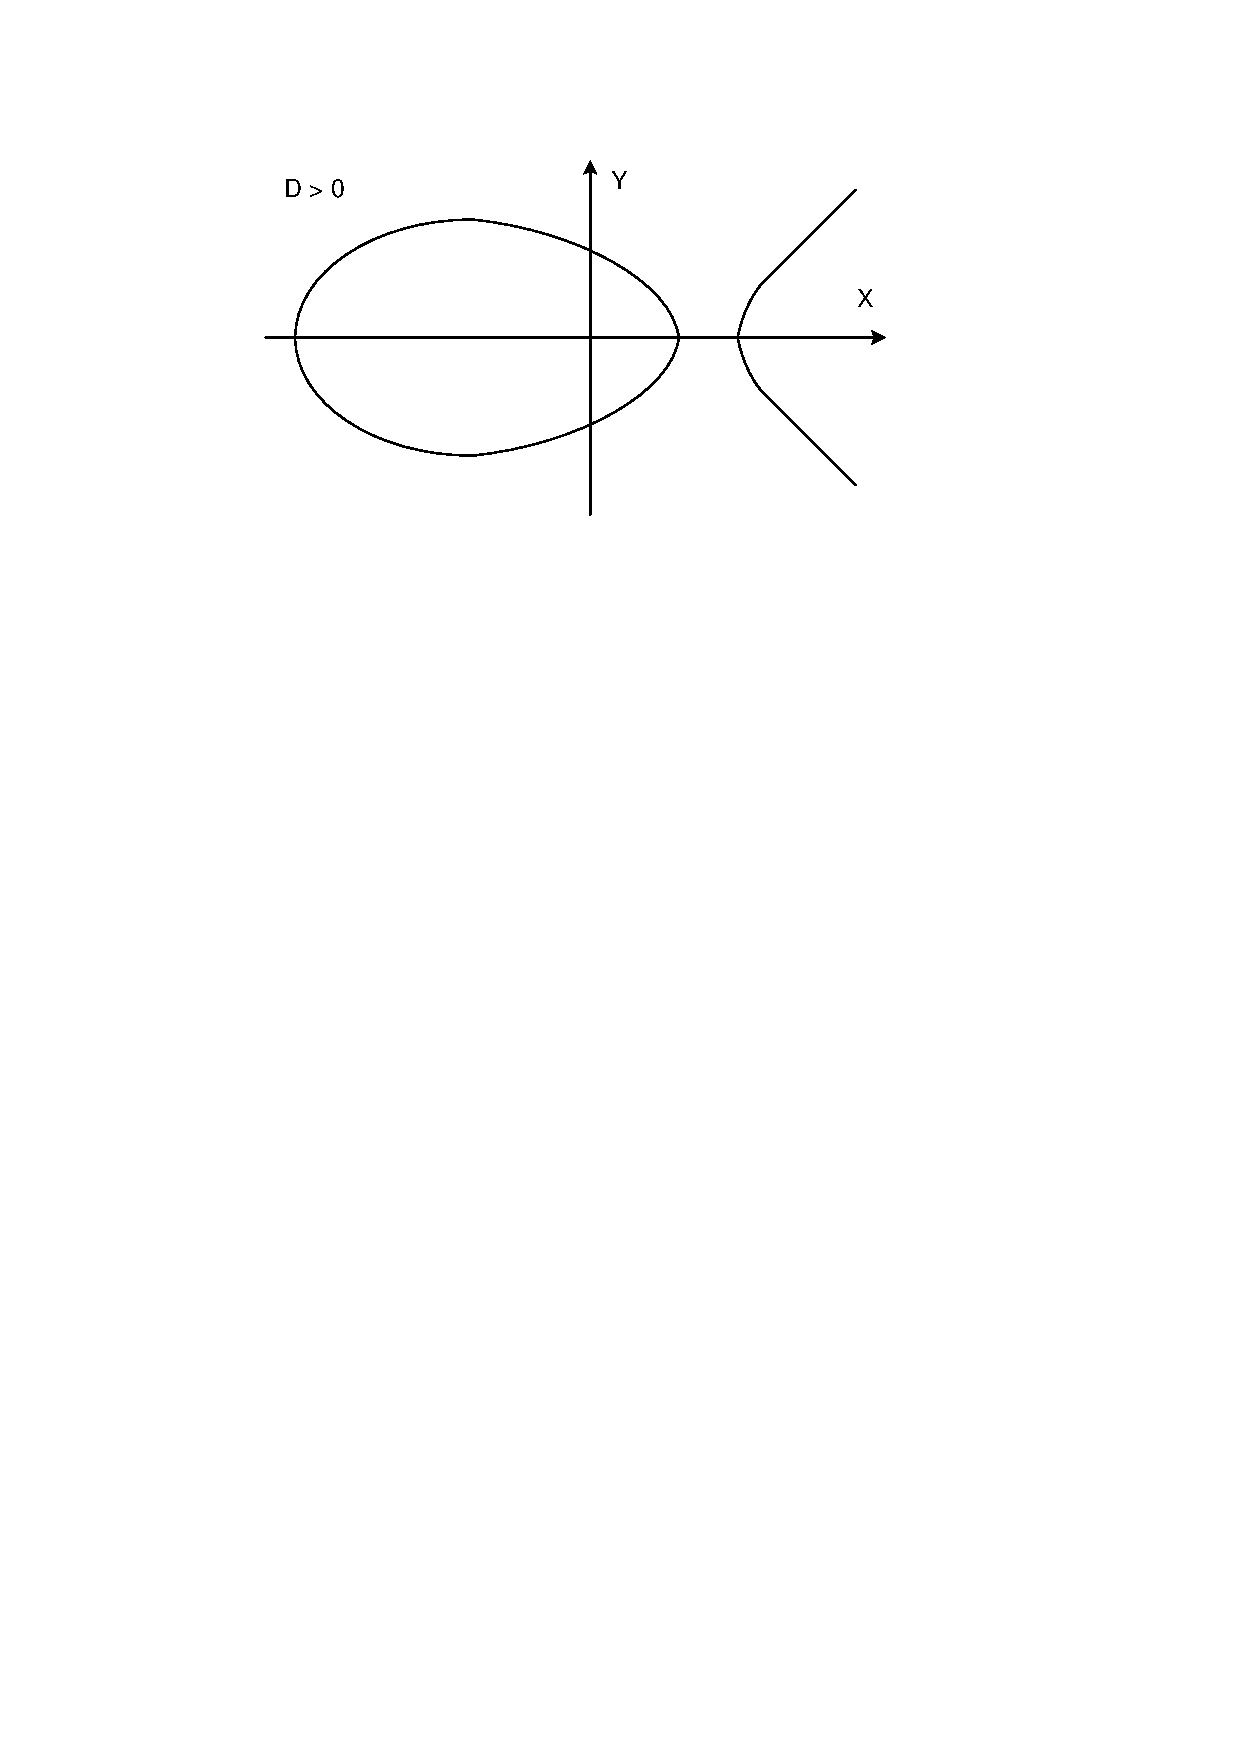
\includegraphics[height=2cm,keepaspectratio]{pic/elliptic-curve-1}}
	~~~~
	\subcaptionbox{$D=0$\label{fig:elliptic-curve-2}}{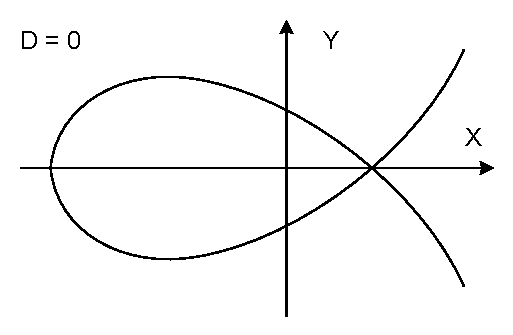
\includegraphics[height=2cm,keepaspectratio]{pic/elliptic-curve-2}}
	~~~~
	\subcaptionbox{$D<0$\label{fig:elliptic-curve-3}}{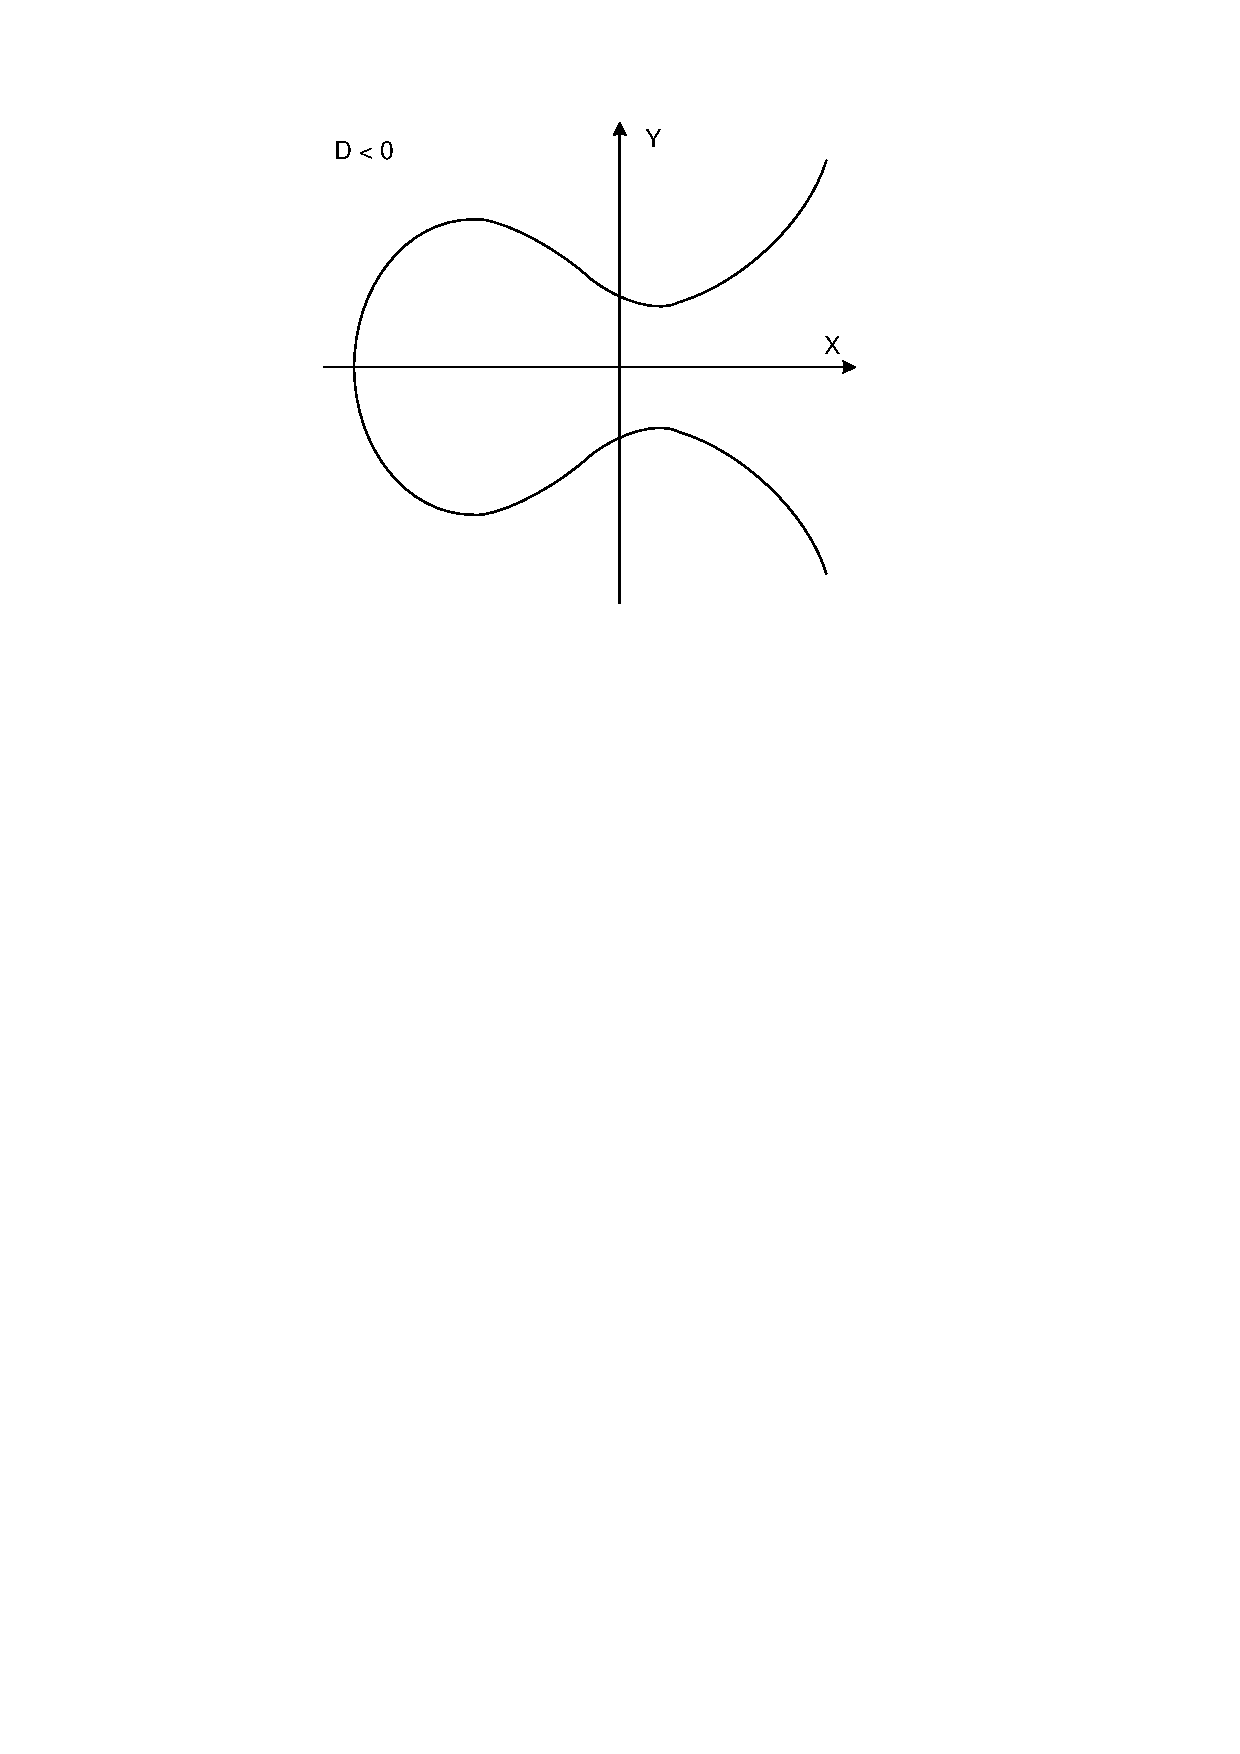
\includegraphics[height=2cm,keepaspectratio]{pic/elliptic-curve-3}}
	\caption{Эллиптические кривые с различными дискриминантами}
\end{figure}

\begin{enumerate}
    \item При $D>0$ график эллиптической кривой состоит из двух частей (см. рис.~\ref{fig:elliptic-curve-1}). Прямая, проходящая через точки $P(x_1; y_1)$ и $Q(x_2; y_2)$, обязательно пересечёт вторую часть кривой в точке с координатами $(x_3; \widetilde{y}_3)$, отображением которой является точка $R(x_3; y_3)$, где $y_3 = - \widetilde{y}_3$. Любые точки на кривой при $D>0$ являются элементами группы по сложению.
    \item Если $D=0$, то левая и правая части касаются в одной точке (см. рис.~\ref{fig:elliptic-curve-2}). Эти кривые называются сингулярными и не рассматриваются.
    \item Если $D<0$, то записанное выше уравнение~\ref{Wer} описывает одну кривую, представленную на рис.~\ref{fig:elliptic-curve-3}.
\end{enumerate}

Рассмотрим операцию сложения точек на эллиптической кривой при $D \ne 0$ (другие кривые не рассматриваются).

Пусть точки $P(x_1; y_1)$ и $Q(x_2; y_2)$ принадлежат эллиптической кривой (рис.~\ref{fig:elliptic-curve-1}). Определим операцию сложения точек
    \[ P + Q = R. \]

\begin{enumerate}
    \item Eсли $P \neq Q$, то точка $R$ определяется как отображение (инвертированная $y$-координата) точки, полученной пересечением эллиптической кривой и прямой $PQ$. Совместно решая уравнения кривой и прямой, можно найти координаты их точки пересечения. Зная координаты точки пересечения, можно вычислить и координаты искомой точки $R = (x_3; y_3)$, которые будут равны:
        \[ x_3 = \lambda^2 - x_1 - x_2, \]
        \[ y_3 = - y_1 + \lambda (x_1 - x_3), \]
где
        \[ \lambda = \frac{y_2 - y_1}{x_2 - x_1} \]
есть тангенс угла наклона между прямой, проходящей через точки $P$ и $Q$, и осью $x$.

	Теперь рассмотрим специальные случаи.
    \item Пусть точки совпадают: $P = Q$. Прямая $PQ$ превращается в касательную к кривой в точке $P$. Находим пересечение касательной с кривой, инвертируем $y$-координату полученной точки, это будет точка $P + P = R$. Тогда $\lambda$ -- тангенс угла между касательной, проведённой к эллиптической кривой в точке $P$, и осью $x$. Запишем уравнение касательной к эллиптической кривой в точке $(x; y)$ в виде:
            \[ 2 y y' = 3 x^2 + a. \]
        Производная равна
            \[ y' = \frac{3 x^2 + a}{2 y}, \]
        и
            \[ \lambda = \frac{3 x_1^2 + a}{2 y_1}. \]
        Координаты $R$ имеют прежний вид:
            \[ x_3 = \lambda^2 - x_1 - x_2, \]
            \[ y_3 = - y_1 + \lambda (x_1 - x_3), \]
    \item Пусть $P$ и $Q$ -- противоположные точки, то есть $P=(x; y)$ и $Q=(x; -y)$. Введём ещё одну точку на бесконечности и обозначим её $O$ (точка $O$ или точка 0 <<ноль>>, или альтернативное обозначение $\infty$). Результатом сложения двух противоположных точек определим точку $O$. Точка $Q$ в данном случае обозначается как $-P$:
        \[ P = (x; y), ~ -P = (x; -y), ~ P + (-P) = O. \]
    \item Пусть $P = (x; 0)$ лежит на оси $x$, тогда
        \[ -P = P, ~ P + P = O. \]
\end{enumerate}

Все точки эллиптической кривой, а также точка $O$ образуют коммутативную группу $\E(\R)$ относительно введённой операции сложения, то есть выполняются законы коммутативной группы\index{группа!точек эллиптической кривой}:
\begin{itemize}
    \item сумма точек $P + Q$ лежит на эллиптической кривой;
    \item существует нулевой элемент -- это точка $O$ на бесконечности:
        \[ \forall P \in \E(\R): ~ O + P = P; \]
    \item для любой точки $P$ существует единственный обратный элемент $-P$:
        \[ P + (-P) = O; \]
    \item выполняется ассоциативный закон:
        \[ (P + Q) + F = P + (Q + F) = P + Q + F; \]
    \item выполняется коммутативный закон:
        \[ P + Q = Q + P. \]
\end{itemize}

Сложение точки с самой собой $d$ раз обозначим как умножение точки на число $d$:
    \[ \underbrace{P + P + \ldots + P}_{d \text{ раз}} = d P. \]


\subsection{Эллиптические кривые над конечным полем}

Эллиптические кривые можно строить не только над полем рациональных чисел, но и над другими полями. То есть координатами точек могут выступать не только числа, принадлежащие полю рациональных чисел $\R$, но и элементы поля комплексных чисел $\mathbb{C}$ или конечного поля $\F$. В криптографии нашли своё применение эллиптические кривые именно над конечными полями.

Далее будем рассматривать эллиптические кривые над конечным полем, являющимся кольцом вычетов по модулю нечётного простого\index{число!простое} числа $p$ (дискриминант не равен 0):
\begin{gather*}
    E: ~ y^2 = x^3 + a x + b, \\
    a, b, x, y \in \Z_p, \\
   \Z_p = \{0, 1, 2, \ldots, p-1\}.
\end{gather*}
Возможна также более компактная запись:
    \[ E: ~ y^2 = x^3 + a x + b \mod p.\]

Точкой эллиптической кривой является пара чисел
    \[ (x; y): x, y \in \Z_p, \]
удовлетворяющая уравнению эллиптической кривой, определённой над конечным полем $\Z_p$.

Операцию сложения двух точек $P = (x_1; y_1)$ и $Q = (x_2; y_2)$ определим точно так же, как и в случае кривой над полем вещественных чисел, описанном выше.

\begin{enumerate}
    \item Две точки $P = (x_1; y_1)$ и $Q = (x_2; y_2)$ эллиптической кривой, определённой над конечным полем $\Z_p$, складываются по правилу:
        \[
            P + Q = R \equiv (x_3; y_3),
        \] \[
            \begin{cases}
                x_3 = \lambda^2 - x_1 - x_2 \mod p,\\
                y_3 = - y_1 + \lambda (x_1 - x_3) \mod p,\\
            \end{cases}
        \]
        где
        \[
            \lambda = \begin{cases}
                \dfrac{y_2 - y_1}{x_2 - x_1} \mod p, & \text{ если } P \ne Q, \\
                \\
                \dfrac{3 x_1^2 + a}{2 y_1} \mod p, & \text{ если } P = Q. \\
            \end{cases}
        \]
    \item Сложение точки $P=(x; y)$ c противоположной \\
        $(-P) = (x; -y)$ даёт точку в бесконечности $O$:
        \begin{gather*}
          P + (-P) = O, \\
         (x_1; y_1) + (x_1; -y_1) = O, \\
         (x_1; 0) + (x_1; 0) = O. 
        \end{gather*}
\end{enumerate}

Мы рассматриваем эллиптические кривые над конечным полем $\Z_p$, где $p > 3$ -- простое\index{число!простое} число, элементы $\Z_p$ -- целые числа $\{0, 1, 2, \ldots, p-1\}$, то есть исследуем следующее уравнение двух переменных $x, y \in \Z_p$:
    \[ y^2 = x^3 + a x + b \mod p, \]
где $a, b \in \Z_p$ -- некоторые константы.

Как и в случае выше, множество точек над конечным полем $\Z_p$, удовлетворяющих уравнению эллиптической кривой, вместе с точкой в бесконечности $O$ образуют конечную группу $\E(\Z_p)$ относительно описанного закона сложения:\index{группа!точек эллиптической кривой}
    \[ \E(\Z_p) ~ \equiv~  O ~ \bigcup ~
        \left\{ (x; y) \in \Z_p \times \Z_p ~\Big|~ y^2 = x^3 + a x + b \mod p \right\}. \]

По теореме Хассе\index{теорема!Хассе} порядок группы точек $|\E(\Z_p)|$ оценивается как
    \[ (\sqrt{p}-1)^2 \leq |\E(\Z_p)| \leq (\sqrt{p}+1)^2, \]
или, в другой записи,
    \[ \Big| |\E(\Z_p)| - p - 1 \Big| \leq 2 \sqrt{p}. \]

\subsection{Примеры группы точек}

\subsubsection{Пример 1}

Пусть эллиптическая кривая задана уравнением
    \[ E: ~ y^2 = x^3 + 1 \mod 7. \]
Найдём все решения этого уравнения, а также количество точек $|\E(\Z_p)|$ на этой эллиптической кривой. Для нахождения решений уравнения составим следующую таблицу:

\begin{center} \begin{tabular}{|c|c|c|c|c|c|c|c|}
    \hline
    $x$ & 0 & 1 & 2 & 3 & 4 & 5 & 6 \\
    \hline
    $y^2$ & 1 & 2 & 2 & 0 & 2 & 0 & 0 \\
    \hline
    $y_1$ & 1 & 3 & 3 & 0 & 3 & 0 & 0 \\
    \hline
    $y_2 = - y_1 \mod p$ & 6 & 4 & 4 &   & 4 &   &   \\
    \hline
\end{tabular} \end{center}

Выпишем все точки, принадлежащие данной эллиптической кривой $\E(\Z_p)$:
\[
    \begin{array}{cccc}
        P_1 = O, & P_2 = (0; 1), & P_3 = (0; 6), & P_4 = (1; 3), \\
        P_5 = (1; 4), & P_6 = (2; 3), & P_7 = (2; 4), & P_8 = (3; 0), \\
        P_9 = (4; 3), & P_{10} = (4; 4), & P_{11} = (5; 0), & P_{12} = (6; 0). \\
    \end{array}
\]

Получили
    \[ |\E(\Z_p)| = 12. \]

Проверим выполнение неравенства Хассе:
    \[ \left| 12 - 7 - 1 \right| = 4 < 2 \sqrt{7}. \]
Следовательно, неравенство Хассе выполняется.

Минимальное натуральное число $s$ такое, что
\[ \underbrace{P + P + \ldots + P}_{s} \equiv s P = O, \]
будем называть \emph{порядком точки $P$}.

%Теорема Лагранжа определяет порядок подгруппы.

\subsubsection{Пример 2}

Группа точек эллиптической кривой
    \[ y^2 = x^3 + 5 x + 6 \mod 17 \]
состоит из точек:
\[ \begin{array}{ccccccc}
    \E(\Z_p) & =~ \Big\{ & (-8; \pm 7), & (-7; \pm 6), & (-6; \pm 7), &   & \\
             &           & (-5; \pm 3), & (-3; \pm 7), & (-1; 0),     & O & \Big\}. \\
\end{array} \]

Порядок группы:
    \[ |\E(\Z_p)| = 12. \]

Порядок группы точек по теореме Хассе:
    \[ (\sqrt{p}-1)^2 \leq |\E(\Z_p)| \leq (\sqrt{p}+1)^2, \]
    \[ 10 \leq 12 \leq 26. \]

Порядки возможных подгрупп: 2, 3, 4, 6 (все возможные делители порядка группы 12).

Найдём порядок точки $A = (-8; 7)$. Так как возможные порядки подгрупп (и всех точек группы) известны, нужно проверить только их.

\begin{itemize}
\item $2A = A + A = (-5; 3)$:
\[\begin{aligned}
& R = P + P, P = (-8; 7), \\
& \lambda = \frac{3 x_P^2 + a}{2y_P} = \frac{3 \cdot (-8)^2 + 5}{2 \cdot 7} = 8 \mod 17, \\
& x_R = \lambda^2 - 2x_P = 8^2 - 2 \cdot (-8) = -5 \mod 17, \\
& y_R = \lambda (x_P - x_R) - y_P = 8 \cdot ((-8) - (-5)) - 7 = 3 \mod 17, \\
& R = (-5; 3). \\
\end{aligned}\]

\item $3A = 2A + A = (-6; 7)$:
\[\begin{aligned}
& R = P + Q, P = (-8; 7), Q = (-5; 3), \\
& \lambda = \frac{y_Q - y_P}{x_Q - x_P} = \frac{3 - 7}{-5 - (-8)} = -7 \mod 17, \\
& x_R = \lambda^2 - x_P - x_Q = (-7)^2 - (-8) - (-5) = -6 \mod 17, \\
& y_R = \lambda (x_P - x_R) - y_P = -7 \cdot (-8 - (-6)) - 7 = 7 \mod 17, \\
& R = (-6; 7). \\
\end{aligned}\]

\item $4A = 2A + 2A = (-5; 3) + (-5; 3) = (-3; 7)$.

\item $6A = 3A + 3A = (-6; 7) + (-6; 7) = (-1; 0)$.

\item $12A = 6A + 6A = (-1; 0) + (-1; 0) = 0$.

\end{itemize}

Найденный порядок точки $A = (-8; 7)$ равен 12, следовательно, она является генератором всей группы.

В таблице~\ref{tab:elliptic-group-sample} найдены порядки точек и циклические подгруппы группы точек $\E(\Z_p)$ такой же эллиптической кривой
    \[ y^2 = x^3 + 5 x + 6 \mod 17. \]
Группа циклическая, число генераторов:
    \[ \varphi(12) = 4. \]
Циклические подгруппы:
    \[ \Gr^{(2)}, ~ \Gr^{(3)}, ~ \Gr^{(4)}, ~ \Gr^{(6)}, \]
верхний индекс обозначает порядок подгруппы.

\begin{table}[!ht]
    \centering
    \caption{Генераторы и циклические подгруппы группы точек эллиптической кривой\label{tab:elliptic-group-sample}}
    \resizebox{\textwidth}{!}{
    \begin{tabular}{|c|l|c|}
        \hline
        Элемент & Порождаемая группа или подгруппа & Порядок \\
        \hline
        $(-8; \pm 7) $ & Вся группа $\E(\Z_p)$ & 12, генератор \\
        $(-7; \pm 6) $ & Вся группа $\E(\Z_p)$ & 12, генератор \\
        $(-6; \pm 7) $ & $\Gr^{(4)} ~=~ \left\{ ~ (-6; \pm 7), ~ (-1; 0), ~ O ~ \right\}$ & 4 \\
        $(-5; \pm 3) $ & $\Gr^{(6)} ~=~ \left\{ ~ (-5; \pm 3), ~ (-3; \pm 7), ~ (-1; 0), ~ O ~ \right\}$ & 6 \\
        $(-3; \pm 7) $ & $\Gr^{(3)} ~=~ \left\{ ~ (-3; \pm 7), ~ O ~ \right\}$ & 3\\
        $(-1; 0)     $ & $\Gr^{(2)} ~=~ \left\{ ~ (-1; 0), ~ O ~ \right\}$ & 2\\
        \hline
    \end{tabular}
    }
\end{table}


\section[Полиномиальные и экспоненциальные алгоритмы]{Полиномиальные и \\ экспоненциальные алгоритмы}

Данный раздел поясняет обоснованность стойкости криптосистем с открытым ключом и имеет лишь косвенное отношение к дискретной математике.

Машина Тьюринга (МТ) (модель, представляющая любой вычислительный алгоритм) состоит из следующих частей:
\begin{itemize}
    \item неограниченная лента, разделённая на клетки; в каждой клетке содержится символ из конечного алфавита, содержащего пустой символ blank; если символ ранее не был записан на ленту, то он считается blank;
    \item печатающая головка, которая может считать, записать символ $a_i$ и передвинуть ленту на 1 клетку влево или вправо $d_k$;
    \item конечная таблица действий
    \[ (q_i, a_j) \rightarrow (q_{i1}, a_{j1}, d_k), \]
где $q$ -- состояние машины.
\end{itemize}

Если таблица переходов однозначна, то машина Тьюринга\index{машина Тьюринга} называется детерминированной. \emph{Детерминированная} машина Тьюринга может \emph{имитировать} любую существующую детерминированную ЭВМ. Если таблица переходов неоднозначна, то есть $(q_i, a_j)$ может переходить по нескольким правилам, то машина \emph{недетерминированная}.

Класс задач $\set{P}$ -- задачи, которые могут быть решены за \emph{полиномиальное} время\index{задача!полиномиальная} на \emph{детерминированной} машине Тьюринга. Пример полиномиальной сложности (количество битовых операций)
    \[ O(k^{\textrm{const}}), \]
где $k$ -- длина входных параметров алгоритма. Операция возведения в степень в модульной арифметике $a^b \mod n$ имеет кубическую сложность $O(k^3)$, где $k$ -- двоичная длина чисел $a,b,n$.

Класс задач $\set{NP}$ -- обобщение класса $\set{P} \subseteq \set{NP}$, включает задачи, которые могут быть решены за \emph{полиномиальное} время на \emph{недетерминированной} машине Тьюринга. Пример сложности задач из $\set{NP}$ -- экспоненциальная сложность\index{задача!экспоненциальная}
    \[ O(\textrm{const}^k). \]
Алгоритм Гельфонда решения задачи дискретного логарифмирования (нахождения $x$ для заданных основания $g$, модуля $p$ и $a = g^x \mod p$), описанный в разделе криптостойкости системы Эль-Гамаля\index{криптосистема!Эль-Гамаля}, имеет сложность $O(e^{k/2})$, где $k$ -- двоичная длина чисел.

В криптографии полиномиальные задачи (относящиеся к классу $\set{P}$) считаются \emph{лёгкими и вычислимыми} на ЭВМ, которые являются детерминированными машинами Тьюринга. Для них, по определению, существуют алгоритмы, работающие за время, полиномиальное относительно размера входных данных. Задачи, относящиеся к классу $\set{NP}$, считаются \emph{трудными и невычислимыми} на ЭВМ, так как все известные на сегодняшний день алгоритмы решения таких задач (в общем случае) требуют экспоненциального времени, а значит всегда можно выбрать такой размер входных данных (читай -- размер ключа шифрования), что время вычисления станет сравнимым с возрастом Вселенной.

Класс $\set{NP}$-полных задач -- подмножество задач из $\set{NP}$, для которых не известен полиномиальный алгоритм для детерминированной машины Тьюринга, и все задачи могут быть сведены друг к другу за полиномиальное время на \emph{детерминированной} машине Тьюринга. Например, задача об укладке рюкзака является $\set{NP}$-полной.

Стойкость криптосистем с \emph{открытым} ключом, как правило, основана на $\set{NP}$ или $\set{NP}$-полных задачах:
\begin{enumerate}
    \item RSA\index{криптосистема!RSA} -- $\set{NP}$-задача факторизации (строго говоря, основана на трудности извлечения корня степени $e$ по модулю $n$).
    \item Криптосистемы типа Эль-Гамаля\index{криптосистема!Эль-Гамаля} -- $\set{NP}$-задача дискретного логарифмирования.
\end{enumerate}

\emph{Нерешённой} проблемой является доказательство неравенства
    \[ \set{P} \neq \set{NP}. \]
Именно на гипотезе о том, что для некоторых задач не существует полиномиальных алгоритмов, и основана стойкость криптосистем с открытым ключом.

\section{Метод индекса совпадений}
\selectlanguage{russian}
\label{chap:coincide-index}

Приведём теоретическое обоснование метода индекса совпадений. Пусть алфавит имеет размер $A$. Пронумеруем его буквы числами от $1$ до $A$. Пусть заданы вероятности появления каждой буквы:
    \[ \mathcal{P} = \left\{ {p_1 ,p_2 , \ldots , p_A } \right\}. \]
В простейшей модели языка предполагается, что тексты состоят из последовательности букв, порождаемых источником независимо друг от друга с известным распределением $\mathcal{P}$.

Найдём индекс совпадений для различных предположений относительно распределений букв последовательности. Сначала рассмотрим случай, когда вероятности всех букв одинаковы. Пусть
    \[ \mathbf{X} = \left[ X_1, X_2, \dots, X_L \right] \]
-- случайный текст с распределением
    \[ \mathcal{P}_1 = \left\{ p_{11}, p_{12}, \dots, p_{1A} \right\}. \]
Найдём индекс совпадений
    \[ I_c(\mathcal{P}_1), \]
то есть вероятность того, что в случайно выбранной паре позиций находятся одинаковые буквы.

Для пары позиций $(k,j)$ найдём условную вероятность $P \left( X_k  = X_j \mid (k,j) \right)$:
    \[ P \left( X_k  = X_j \mid (k,j) \right) ~=~ \sum\limits_{i=1}^A p_{1i}^2 ~\equiv~ k_{p_1}. \]
Эта вероятность не зависит от выбора пары позиций $(k,j)$.

Так как число различных пар равно $\frac{L(L - 1)}{2}$, то вероятность случайного выбора пары $(k,j)$ равна
    \[ P_{(K,J)} (k,j) = \frac{2}{L(L - 1)}. \]
Следовательно,
\begin{multline*}
    I(\mathcal{P}_1) ~= \sum \limits_{1 \leq k < j \leq L} P_{(K,J)}(k,j) ~\cdot~ P(X_k  = X_j \mid (k,j)) =\\
    = \sum \limits_{1 \leq k < j \leq L} \frac{2}{L(L - 1)} k_{p_1} = k_{p_1}.
\end{multline*}

Найдём теперь аналогичную вероятность $I\left( {\mathcal{P}_1 ,\mathcal{P}_2 } \right)$ для случая, когда последовательность независимых случайных букв может быть представлена в виде
\[
\mathbf{X} = \left[ {\begin{array}{*{20}c}
   {X_1 ,}  \\
   {Y_1 ,}  \\
 \end{array} \begin{array}{*{20}c}
   {X_2 ,}  \\
   {Y_2 ,}  \\
 \end{array} \begin{array}{*{20}c}
   { \ldots ,}  \\
   { \ldots ,}  \\
 \end{array} \begin{array}{*{20}c}
   {X_{L/2} }  \\
   {Y_{L/2} }  \\
 \end{array} } \right],
\]
где одинаково распределённые случайные буквы в первой строке имеют распределение:
    \[ \mathcal{P}_1  = \left\{ {p_{11} ,p_{12} , \ldots , p_{1A} } \right\}, \]
а одинаково распределённые случайные буквы во второй строке имеют другое распределение:
    \[ \mathcal{P}_2  = \left\{ {p_{21} ,p_{22} , \ldots , p_{2A} } \right\}. \]

В этом случае сумму по всем парам мы разделяем на три суммы: по парам внутри позиций первой строки, по парам внутри позиций второй строки и по парам, в которых первая позиция берётся из первой строки, а вторая -- из второй:
\begin{multline*}
I(\mathcal{P}_1, \mathcal{P}_2) =
        \frac{2}{L(L - 1)} \cdot \left(
        \sum \limits_{1 \leq k < j \leq L/2} P( X_k  = X_j \mid ( k,j )) + \right.
\\
        \left. + \sum\limits_{1 \leq k < j \leq L/2} P(Y_k  = Y_j \mid (k,j)) +
            \sum\limits_{k=1}^{L/2} \sum\limits_{j=1}^{L/2} {P(X_k = Y_j \mid (k,j))} \right) =
\\
    = \frac{2}{L(L - 1)} \left( \frac{1}{2} \frac{L}{2} \left( \frac{L}{2} - 1 \right) k_{p_1} +
        \frac{1}{2} \frac{L}{2} \left( \frac{L}{2} - 1 \right) k_{p_2} +
        \left( \frac{L}{2} \right)^2 k_{p_1, p_2} \right),
\end{multline*}
где обозначено
    \[ k_{p_1, p_2}  = \sum\limits_{i=1}^A p_{1,i} p_{2,i}. \]

В общем случае рассмотрим последовательность, представленную в виде матрицы, состоящей из $m$ строк и $\frac{L}{m}$ столбцов, где
\[
{\mathbf X} = \left[ {\begin{array}{*{20}c}
   {X_1 } & {X_2 } &  \cdots  & {X_{L/m} }  \\
   {Y_1 } & {Y_2 } &  \cdots  & {Y_{L/m} }  \\
    \vdots  &  \vdots  &  \ddots  &  \vdots   \\
   {Z_1 } & {Z_2 } &  \cdots  & {Z_{L/m} }  \\
\end{array}} \right].
\]

Считаем, что одинаково распределённые случайные буквы в первой строке имеют распределение
    \[ P_1  = \left\{ {p_{11} ,p_{12} , \ldots , p_{1A} } \right\}, \]
одинаково распределённые случайные буквы во второй строке имеют распределение
    \[ P_2  = \left\{ {p_{21} ,p_{22} , \ldots , p_{2A} } \right\} \]
и~т.\,д., одинаково распределённые случайные буквы $m$-й строки имеют распределение
    \[ P_m  = \left\{ {p_{m1},p_{m2} , \ldots , p_{mA} } \right\}. \]

Для вычисления вероятности того, что в случайно выбранной паре позиций будут одинаковые буквы, выполним суммирование по различным парам внутри строк и по парам между различными строками. Аналогично предыдущему случаю получим:
\begin{multline*}
I(\mathcal{P}_1, \mathcal{P}_2, \ldots, \mathcal{P}_m ) = \\
= \frac{2}{L(L - 1)} \left( \frac{L}{2m} \left( \frac{L}{m} - 1 \right) k_{p_1} + \frac{L}{2m} \left( \frac{L}{m} - 1 \right) k_{p_2} + \right. \\
+ \dots + \left. \frac{L}{2m} \left( \frac{L}{m} - 1 \right) k_{p_m} \right) + \\
+ \frac{2}{L(L - 1)} \left( \left( \frac{L}{m} \right)^2 k_{p_1, p_2} + \left( \frac{L}{m} \right)^2 k_{p_1, p_3} + \dots + \left( \frac{L}{m} \right)^2 k_{p_{m - 1}, p_m } \right).
\end{multline*}

Первая сумма содержит $m$ слагаемых, вторая -- $ \frac{m(m-1)}{2}$ слагаемых. Полагая
    \[ k_{p_1} = k_{p_2} = \dots = k_{p_m} = k_p, \]
    \[ k_{p_i p_j } = k_r = \frac{1}{A}, ~ i \ne j, \]
получим после несложных выкладок
    \[ m = \frac{k_p  - k_r}{I - k_r  + \frac{k_p  - I}{L}}. \]


\chapter{Примеры задач}
\selectlanguage{russian}
\taskinit

В данном разделе приведены примеры задач, которые использовались на контрольных работах в МФТИ по курсу <<Защита информации>> в 2011--2015 годах.

\section{Математические основы}
\tasksection

\tasknumber Найдите общее количество генераторов аддитивной циклической группы $\mathbb{Z}_{33}$ с операцией в виде сложения чисел по модулю 33 и перечислите их.
\medbreak
\textbf{Ответ:} 20: [1, 2, 4, 5, 7, 8, 10, 13, 14, 16, 17, 19, 20, 23, 25, 26, 28, 29, 31, 32].
\bigbreak

\tasknumber Вычислить в поле Галуа $GF\left( {2^{5} } \right)$, $m\left( x \right) = x^{5} + x^{3} + x^{2} + x + 1$, следующее значение: $28 \times 29 + 23^2$. Многочлены заданы как десятичное представление двоичных коэффициентов, свободный член многочлена соответствует младшему биту двоичного представления. В ответе привести в десятичном представлении результаты умножения, возведения в степень и сложения.
\medbreak
\textbf{Решение:}
\begin{itemize}\itemsep1pt \parskip0pt \parsep0pt
	\item $a = "28" \Rightarrow a\left( x \right) = x^{4} + x^{3} + x^{2}$;
	\item $b = "29" \Rightarrow b\left( x \right) = x^{4} + x^{3} + x^{2} + 1$;
	\item $c = "23" \Rightarrow c\left( x \right) = x^{4} + x^{2} + x + 1$;
	\item $a \left( x \right) \times b \left( x \right) = x^{4} + x^{3} + x + 1 \Rightarrow a \times b = "27"$;
	\item $c \left( x \right)^2 = x^{4} + x^{3} + x^{2} \Rightarrow c^2 = "28"$;
	\item $result\left( x \right) = x^{2} + x + 1 \Rightarrow result = "7"$.
\end{itemize}
\medbreak
\textbf{Ответ:} <<27>>; <<28>>; <<7>>.
\bigbreak

\tasknumber Вычислить в поле Галуа $GF\left( 27 \right)$, $m\left( x \right) = x^{3} + x^{2} + x + 2$, следующее значение: $26 \times 11 + 25^2$. Многочлены заданы как десятичное представление троичных коэффициентов, свободный член многочлена соответствует младшему триту троичного представления. В ответе привести в десятичном представлении результаты умножения, возведения в степень и сложения.
\medbreak
\textbf{Решение:}
\begin{itemize}\itemsep1pt \parskip0pt \parsep0pt
	\item $a = "26" \Rightarrow a\left( x \right) = 2 x^{2} + 2 x + 2$;
	\item $b = "11" \Rightarrow b\left( x \right) = x^{2} + 2$;
	\item $c = "25" \Rightarrow c\left( x \right) = 2 x^{2} + 2 x + 1$;
	\item $a \left( x \right) \times b \left( x \right) = x^{2} + 1 \Rightarrow a \times b = "10"$;
	\item $c ^2\left( x \right) = x + 2 \Rightarrow c^2 = "5"$;
	\item $result\left( x \right) = x^{2} + x \Rightarrow result = "12"$.
\end{itemize}
\medbreak
\textbf{Ответ:} <<10>>; <<5>>; <<12>>.
\bigbreak

\tasknumber Используя алгоритм быстрого возведения в степень (с помощью разложения показателя степени по степеням двойки по схеме <<слева направо>>), вычислить ${175}^{235} \mod {257}$.
\medbreak
\textbf{Решение:}
\begin{itemize}\itemsep1pt \parskip0pt \parsep0pt
	\item двоичная форма записи степени: $235_{10} = 11101011_{2}$;
	\item полное выражение для вычисления: $(((((((1 \times {175}^1)^2 \times {175}^1)^2 \times {175}^1)^2 \times {175}^0)^2 \times {175}^1)^2 \times {175}^0)^2 \times {175}^1)^2 \times {175}^1\mod 257$;
	\item шаг \No1: $1^2 \times 175 \mod 257  = 175$;
	\item шаг \No2: $175^2 \times 175 \mod 257 = 154$;
	\item шаг \No3: $154^2 \times 175 \mod 257 = 7$;
	\item шаг \No4: $7^2 \mod 257 = 49 \mod 257 = 49$;
	\item шаг \No5: $49^2 \times 175 \mod 257 = 237$;
	\item шаг \No6: $237^2 \mod 257 = 143$;
	\item шаг \No7: $143^2 \times 175 \mod 257 = 107$;
	\item шаг \No8: $107^2 \times 175 \mod 257 = 3$.
\end{itemize}
\medbreak
\textbf{Ответ:} 3.
\bigbreak

\section{Общие определения и теория}
\tasksection

\tasknumber Рассмотрим множество паролей, состоящих из 12 строчных и заглавных латинских букв, а также цифр.
\begin{itemize}\itemsep1pt \parskip0pt \parsep0pt
\item Каков размер этого множества?
\item Сколько времени потребуется на взлом шифртекста, зашифрованного данным паролем, если предположить, что во взломе участвуют все компьютеры мира (7~млрд.), а средний компьютер перебирает 300~000 паролей в секунду?\footnote{См. скорости перебора MD5-хэшей\index{хэш-функция!MD5} на странице \texttt{http://openwall.info\hspace{0pt}/wiki\hspace{0pt}/john\hspace{0pt}/benchmarks}.}
\item Каковы затраты электроэнергии в денежном эквиваленте, если средний компьютер потребляет мощность 400~Вт, а стоимость 1~кВт$\times$час составляет 4,68~рубля?
\end{itemize}
\medbreak
\textbf{Решение:}
\begin{itemize}\itemsep1pt \parskip0pt \parsep0pt
	\item общее количество символов: $26 + 26 + 10 = 62$;
	\item общее количество паролей: $62^{12} \approx 3{,}226\times 10^{21}$;
	\item время на перебор: $62^{12} / (3 \times 10^5) / (7 \times 10^9 ) \approx 1{,}54 \times 10^{6}$ сек.;
	\begin{itemize}\itemsep1pt \parskip0pt \parsep0pt
		\item в минутах: $\approx 25605$;
		\item в часах: $\approx 427$;
		\item в днях: $\approx 18$;
	\end{itemize}
	\item стоимость: $427 \times (7 \times 10^9 ) \times 0{,}4 \times 4{,}68 \approx 5{,}59 \times 10^{12}$ руб.
\end{itemize}
\medbreak
\textbf{Ответ:} паролей $3{,}226 \times 10^{21}$; на перебор нужно $1{,}54 \times 10^6$ секунд ($\approx 18$ дней); затраты -- 5,6 триллиона рублей.
\bigbreak

\tasknumber Источник открытого текста характеризуется случайной величиной $X$, принимающей два значения $x_1$ и $x_2$ с вероятностями $p \left( x = x_1 \right) = 1/5$ и $p \left( x = x_2 \right) = 4/5$ соответственно. Источник ключей характеризуется случайной величиной $Z$, независимой от величины $X$, принимающей два значения $z_1$ и $z_2$ с вероятностями $p \left( z = z_1 \right) = 1/6$ и $p \left( z = z_2 \right) = 5/6$ соответственно. Функция шифрования $E_{z} \left( x \right)$ задаётся следующими правилами: $\left( x_1, z_1 \right) \to y_1$, $\left( x_1, z_2 \right) \to y_2$, $\left( x_2, z_1 \right) \to y_2$, $\left( x_2, z_2 \right) \to y_1$.
\begin{enumerate}\itemsep1pt \parskip0pt \parsep0pt
	\item Найдите собственную информацию каждого из сообщений открытого текста в битах.
	\item Найдите энтропию источника сообщений, источника ключей и шифртекста в битах.
	\item Найдите взаимную информацию открытого текста и ключа в битах.
	\item Найдите взаимную информацию открытого текста и шифртекста в битах.
	\item Найдите взаимную информацию ключа и шифртекста в битах.
	\item Найдите апостериорное распределение вероятностей открытого текста для обоих вариантов перехваченных злоумышленником шифртекстов $y_1$ и $y_2$. Используя вычисленные значения, определите, является ли данная шифросистема абсолютно надёжной. Если нет, то что в данной криптосистеме необходимо поменять? Покажите, что апостериорные вероятности после доработки будут удовлетворять необходимым требованиям абсолютно надёжной криптосистемы.
\end{enumerate}
\medbreak
\textbf{Ответ:}
\begin{itemize}\itemsep1pt \parskip0pt \parsep0pt
	\item $I \left( x_1 \right) = \log_2 5 = 2{,}322$ бит; $I \left( x_2 \right) = \log_2 5/4 = 0{,}322$ бит;
	\item $H \left( X \right) = 0{,}722$ бит; $H \left( Z \right) = 0{,}650$ бит; $H \left( Y \right) = 0{,}881$ бит;
	\item $I \left( X ; Z \right) = 0$ бит; $I \left( X; Y \right) = 0{,}231$ бит; $I \left( Y; Z \right) = 0{,}159$ бит;
	\item $p \left( x_1 | y_1 \right) = 1/21$; $p \left( x_2 | y_1 \right) = 20/21$; $p \left( x_1 | y_2 \right) = 5/9$; $p \left( x_2 | y_2 \right) = 4/9$; не является.
\end{itemize}

\section{КСГПСЧ и потоковые шифры}
\tasksection

\tasknumber Привести следующие два элемента последовательности, сформированной линейным конгруэнтным методом, если предыдущие 3 элемента последовательности такие: 348, 65, 139, а все вычисления выполняются в поле $\mathbb{F}_{499}$.
\medbreak
\textbf{Решение:}
\begin{itemize}\itemsep1pt \parskip0pt \parsep0pt
	\item используя предыдущие значения выхода генератора, строим систему уравнений:
		\[\left\{ {\begin{array}{*{20}c}
		348 \cdot a + c = 65 \mod 499 \\
		65 \cdot a + c = 139 \mod 499 \\
		\end{array} } \right. ;\]
	\item из системы уравнений находим $a = 467$ и $c = 223$;
	\item используя найденные значения, находим следующие элементы последовательности:
	\begin{itemize}\itemsep1pt \parskip0pt \parsep0pt
		\item $x_{3} = a x_{2} + c \mod m = 467 \cdot 139 + 223 \mod 499 = 266$;
		\item $x_{4} = a x_{3} + c \mod m = 467 \cdot 266 + 223 \mod 499 = 194$.
	\end{itemize}
\end{itemize}
\medbreak
\textbf{Ответ:} 266, 194.
\bigbreak

\tasknumber Приведите \emph{предыдущие} 5 бит выхода генератора псевдослучайной последовательности, основанного на регистре сдвига с линейной обратной связью, если известно, что характеристический полином регистра -- $m\left(x\right)=x^{5} + x^{3} + 1$ (см. рис.), а дальнейшая последовательность такова: $1, 1, 0, 1, 0, 1$.
\begin{center}
	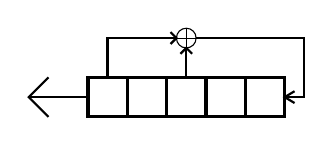
\begin{tikzpicture}[scale=0.05]
		\draw[black,very thick] (30,30) -- (30,40) -- (40,40) -- (40,30) -- (30,30) -- (30,40);
		\draw[black,thick] (35,40) -- (35,50) -- (35,50) -- (37.5,50);
		\draw[black,very thick] (40,30) -- (40,40) -- (50,40) -- (50,30) -- (40,30) -- (40,40);
		\draw[black,very thick] (50,30) -- (50,40) -- (60,40) -- (60,30) -- (50,30) -- (50,40);
		\draw[black,thick] (55,40) -- (55,47.5);
		\draw[black,thick] (53.5,46) -- (55,47.5) -- (56.5,46);
		\draw[black,thick] (37.5,50) -- (52.5,50);
		\draw[black,thick] (51,51.5) -- (52.5,50) -- (51,48.5);
		\draw (55,50) circle [radius=2.5];
		\draw[black] (52.5,50) -- (57.5,50);
		\draw[black] (55,47.5) -- (55,52.5);
		\draw[black,very thick] (60,30) -- (60,40) -- (70,40) -- (70,30) -- (60,30) -- (60,40);
		\draw[black,very thick] (70,30) -- (70,40) -- (80,40) -- (80,30) -- (70,30) -- (70,40);
		\draw[black,thick] (57.5,50) -- (85,50) -- (85,35) -- (80,35);
		\draw[black,thick] (82.5,36.5) -- (80,35) -- (82.5,33.5);
		\draw[black,thick] (30,35) -- (15,35);
		\draw[black,thick] (20,30) -- (15,35) -- (20,40);
	\end{tikzpicture}
\end{center}
\medbreak
\textbf{Решение.}
\begin{itemize}\itemsep1pt \parskip0pt \parsep0pt
	\item Из коэффициентов многочлена $m\left(x\right)$ получаем формулу предыдущего элемента:
		\[ m\left(x\right) = \sum\limits_{i = 5 \dots 1} {a_i x^i } + 1 = x^{5} + x^{3} + 1; \]
		\[ b_0 = a_5 b_5 \oplus \dots \oplus a_1 b_1 = b_{5} \oplus b_{3}.\]
		Это формула бита, который на следующей итерации станет битом $b_1$, то есть значение функции обратной связи регистра;
	\item $b_5 = b_0\oplus b_{3}$ -- формула выходного бита, если известны остальные биты и значение функции обратной связи;
	\item За счёт последних 5 бит выхода восстанавливаем состояние регистра $\overrightarrow{s_{1}}=\left(b_{1}, b_{2}, b_{3}, b_{4}, b_{5}\right) = \left(1, 0, 1, 0, 1\right)$. Далее начинаем отматывать время назад.
	\item $\overrightarrow{s_{1}}=\left(1, 0, 1, 0, 1\right)$. $\overrightarrow {s_{0}} = \left(0, 1, 0, 1, ? \right)$ и $b_0 = 1$. \\
		$b_5 = b_0\oplus b_{3}=1 \oplus 0=1$. $\overrightarrow{s_{0}}=\left(0, 1, 0, 1, 1\right)$. \\
		Выход — 1;
	\item $\overrightarrow{s_{0}}=\left(0, 1, 0, 1, 1\right)$. $\overrightarrow {s_{-1}} = \left(1, 0, 1, 1, ? \right)$ и $b_0 = 0$. \\
		$b_5 = b_0\oplus b_{3}=0 \oplus 1=1$. $\overrightarrow{s_{-1}}=\left(1, 0, 1, 1, 1\right)$. \\
		Выход — 1;
	\item $\overrightarrow{s_{-1}}=\left(1, 0, 1, 1, 1\right)$. $\overrightarrow {s_{-2}} = \left(0, 1, 1, 1, ? \right)$ и $b_0 = 1$. \\
		$b_5 = b_0\oplus b_{3}=1 \oplus 1=0$. $\overrightarrow{s_{-2}}=\left(0, 1, 1, 1, 0\right)$. \\
		Выход — 0;
	\item $\overrightarrow{s_{-2}}=\left(0, 1, 1, 1, 0\right)$. $\overrightarrow {s_{-3}} = \left(0, 0, 1, 1, ? \right)$ и $b_0 = 0$. \\
		$b_5 = b_0\oplus b_{3}=0 \oplus 1=1$. $\overrightarrow{s_{-3}}=\left(1, 1, 1, 0, 1\right)$. \\
		Выход — 1;
	\item $\overrightarrow{s_{-3}}=\left(1, 1, 1, 0, 1\right)$. $\overrightarrow {s_{-4}} = \left(0, 1, 0, 1, ? \right)$ и $b_0 = 1$. \\
		$b_5 = b_0\oplus b_{3}=1 \oplus 0=1$. $\overrightarrow{s_{-4}}=\left(1, 1, 0, 1, 1\right)$. \\
		Выход — 1;
	\item $\overrightarrow{s_{-4}}=\left(1, 1, 0, 1, 1\right)$. $\overrightarrow {s_{-5}} = \left(0, 1, 1, 0, ? \right)$ и $b_0 = 1$. \\
		$b_5 = b_0\oplus b_{3}=1 \oplus 1=0$. $\overrightarrow{s_{-5}}=\left(1, 0, 1, 1, 0\right)$. \\
		Выход — 0;
	\item Ответ (в порядке выдачи бит генератором): $0, 1, 1, 0, 1$.
	\item Краткое оформление второй части задачи можно увидеть в таблице~\ref{table:task-lfsr-1-short-solution}. Таблица заполняется снизу вверх (так как нам нужны предыдущие биты, а не следующие). Последняя строка таблицы соответствует последнему известному состоянию регистра -- последним 5 битам последовательности. Столбцы таблицы связаны формулой $b_{5} \oplus b_{3} = b_0 $. Ответ находится в первых 5 элементах первого столбца.
	\begin{table}[!thb]
		\centering
		\begin{tabular}{ l | c || c c c c c|| c }
		 & & $b_{5}$& $b_{4}$& $b_{3}$& $b_{2}$& $b_{1}$ & $b_0$ \\
		  \hline
		  $\overrightarrow {s_{-5}}$ & 0 & 0 & 1 & 1 & 0 & 1& 1 \\
		  $\overrightarrow {s_{-4}}$ & 1 & 1 & 1 & 0 & 1 & 1& 1 \\
		  $\overrightarrow {s_{-3}}$ & 1 & 1 & 0 & 1 & 1 & 1& 0 \\
		  $\overrightarrow {s_{-2}}$ & 0 & 0 & 1 & 1 & 1 & 0& 1 \\
		  $\overrightarrow {s_{-1}}$ & 1 & 1 & 1 & 1 & 0 & 1& 0 \\
		  $\overrightarrow {s_{0}}$ & 1 & 1 & 1 & 0 & 1 & 0& 1 \\
		  $\overrightarrow {s_{1}}$ & 1 & 1 & 0 & 1 & 0 & 1& $\cdot$ \\
		\hline
		\end{tabular}
		\caption{Краткое оформление решения задачи \No\arabic{task-section}.\arabic{task-number} в виде таблицы}
		\label{table:task-lfsr-1-short-solution}
	\end{table}
\end{itemize}
\medbreak
\textbf{Ответ:} $0, 1, 1, 0, 1$.
\bigbreak

\tasknumber Укажите характеристический полином и приведите следующие 5 бит выхода генератора псевдослучайной последовательности, основанного на регистре сдвига с линейной обратной связью, если известно, что степень характеристического полинома регистра -- $m\left(x\right)$ -- равна 5, а предыдущая последовательность такова: $0, 1, 0, 0, 1, 1, 0, 0, 0, 0, 1$. Порядок бит в последовательности соответствует порядку их генерации РСЛОС.
\medbreak
\textbf{Решение.}
\begin{itemize}\itemsep1pt \parskip0pt \parsep0pt
	\item Каждый бит выходной последовательности есть функция 5 предыдущих выходных бит вида $b_0 = f\left( b_{5} \dots b_1 \right) $. В данных обозначениях $b_{5}$ является наиболее ранним битом, а $b_1$ -- последним, который сгенерировал РСЛОС непосредственно перед генерацией бита $b_0$.  Вид функции задаётся характеристическим многочленом, который и нужно найти.
	\[\begin{array}{l}
		m \left( x \right) = x^{5} +  a_{4} x^{4} + a_{3} x^{3} + a_{2} x^{2} + a_{1} x^{1} +1; \\
		b_{5} \oplus a_{4} b_{4} \oplus a_{3} b_{3} \oplus a_{2} b_{2} \oplus a_{1} b_{1} = b_0. \\
	\end{array}\]
	\[\begin{array}{l}
		f\left(0,1,0,0,1\right) = 1, \\
		f\left(1,0,0,1,1\right) = 0, \\
		f\left(0,0,1,1,0\right) = 0, \\
		f\left(0,1,1,0,0\right) = 0, \\
		f\left(1,1,0,0,0\right) = 0, \\
		f\left(1,0,0,0,0\right) = 1. \\
	\end{array}\]
	\item Это приводит к системе уравнений:
	\[\left\{ {\begin{array}{*{20}c}
		f\left(0,1,0,0,1\right) = 0 \oplus \left( a_{4} \cdot 1\right) \oplus \left( a_{3} \cdot 0\right) \oplus \left( a_{2} \cdot 0\right) \oplus \left( a_{1} \cdot 1\right) = 1 \\
		f\left(1,0,0,1,1\right) = 1 \oplus \left( a_{4} \cdot 0\right) \oplus \left( a_{3} \cdot 0\right) \oplus \left( a_{2} \cdot 1\right) \oplus \left( a_{1} \cdot 1\right) = 0 \\
		f\left(0,0,1,1,0\right) = 0 \oplus \left( a_{4} \cdot 0\right) \oplus \left( a_{3} \cdot 1\right) \oplus \left( a_{2} \cdot 1\right) \oplus \left( a_{1} \cdot 0\right) = 0 \\
		f\left(0,1,1,0,0\right) = 0 \oplus \left( a_{4} \cdot 1\right) \oplus \left( a_{3} \cdot 1\right) \oplus \left( a_{2} \cdot 0\right) \oplus \left( a_{1} \cdot 0\right) = 0 \\
		f\left(1,1,0,0,0\right) = 1 \oplus \left( a_{4} \cdot 1\right) \oplus \left( a_{3} \cdot 0\right) \oplus \left( a_{2} \cdot 0\right) \oplus \left( a_{1} \cdot 0\right) = 0 \\
		f\left(1,0,0,0,0\right) = 1 \oplus \left( a_{4} \cdot 0\right) \oplus \left( a_{3} \cdot 0\right) \oplus \left( a_{2} \cdot 0\right) \oplus \left( a_{1} \cdot 0\right) = 1 \\
	\end{array} } \right.\]
	\[\left\{ {\begin{array}{*{20}l}
		a_{4} \oplus a_{1} = 1 \\
		a_{2} \oplus a_{1} = 1 \\
		a_{3} \oplus a_{2} = 0 \\
		a_{4} \oplus a_{3} = 0 \\
		a_{4} = 1 \\
	\end{array} } \right.\]
	\item Найденные из системы уравнения коэффициенты $\left(a_{4}, a_{3}, a_{2}, a_{1}\right) = \left(1 , 1 , 1 , 0\right)$.
	\item Характеристический полином регистра:
		\[\begin{array}{l}
			m \left( x \right) = x^{5}+ a_{4} x^{4}+ a_{3} x^{3}+ a_{2} x^{2}+ a_{1} x^{1} + 1; \\
			m = x^{5} + x^{4} + x^{3} + x^{2} + 1. \\
		\end{array}\]
	\item Схема РСЛОС приведена на рисунке.
	\begin{center}
		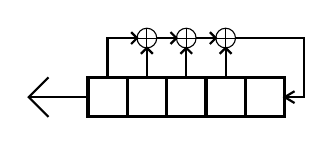
\begin{tikzpicture}[scale=0.05]
			\draw[black,very thick] (30,30) -- (30,40) -- (40,40) -- (40,30) -- (30,30) -- (30,40);
			\draw[black,thick] (35,40) -- (35,50) -- (35,50) -- (37.5,50);
			\draw[black,very thick] (40,30) -- (40,40) -- (50,40) -- (50,30) -- (40,30) -- (40,40);
			\draw[black,thick] (45,40) -- (45,47.5);
			\draw[black,thick] (43.5,46) -- (45,47.5) -- (46.5,46);
			\draw[black,thick] (37.5,50) -- (42.5,50);
			\draw[black,thick] (41,51.5) -- (42.5,50) -- (41,48.5);
			\draw (45,50) circle [radius=2.5];
			\draw[black] (42.5,50) -- (47.5,50);
			\draw[black] (45,47.5) -- (45,52.5);
			\draw[black,very thick] (50,30) -- (50,40) -- (60,40) -- (60,30) -- (50,30) -- (50,40);
			\draw[black,thick] (55,40) -- (55,47.5);
			\draw[black,thick] (53.5,46) -- (55,47.5) -- (56.5,46);
			\draw[black,thick] (47.5,50) -- (52.5,50);
			\draw[black,thick] (51,51.5) -- (52.5,50) -- (51,48.5);
			\draw (55,50) circle [radius=2.5];
			\draw[black] (52.5,50) -- (57.5,50);
			\draw[black] (55,47.5) -- (55,52.5);
			\draw[black,very thick] (60,30) -- (60,40) -- (70,40) -- (70,30) -- (60,30) -- (60,40);
			\draw[black,thick] (65,40) -- (65,47.5);
			\draw[black,thick] (63.5,46) -- (65,47.5) -- (66.5,46);
			\draw[black,thick] (57.5,50) -- (62.5,50);
			\draw[black,thick] (61,51.5) -- (62.5,50) -- (61,48.5);
			\draw (65,50) circle [radius=2.5];
			\draw[black] (62.5,50) -- (67.5,50);
			\draw[black] (65,47.5) -- (65,52.5);
			\draw[black,very thick] (70,30) -- (70,40) -- (80,40) -- (80,30) -- (70,30) -- (70,40);
			\draw[black,thick] (67.5,50) -- (85,50) -- (85,35) -- (80,35);
			\draw[black,thick] (82.5,36.5) -- (80,35) -- (82.5,33.5);
			\draw[black,thick] (30,35) -- (15,35);
			\draw[black,thick] (20,30) -- (15,35) -- (20,40);
		\end{tikzpicture}
	\end{center}
	\item Теперь, когда характеристический полином известен, восстанавливаем состояния регистра по последним 5 выходным битам:
	\begin{itemize}\itemsep1pt \parskip0pt \parsep0pt
		\item $\left(b_{5}, b_{4}, b_{3}, b_{2}, b_{1}\right) = \left(0, 0, 0, 0, 1\right)$. Сумма: $b_0 = b_{5} \oplus b_{4} \oplus b_{3} \oplus b_{2}=0 \oplus 0 \oplus 0 \oplus 0=0$. Следующее состояние $\left(0, 0, 0, 1, 0\right)$, а текущий выход $b_{5}=0$.
		\item $\left(b_{5}, b_{4}, b_{3}, b_{2}, b_{1}\right) = \left(0, 0, 0, 1, 0\right)$. Сумма: $b_0 = b_{5} \oplus b_{4} \oplus b_{3} \oplus b_{2}=0 \oplus 0 \oplus 0 \oplus 1=1$. Следующее состояние $\left(0, 0, 1, 0, 1\right)$, а текущий выход $b_{5}=0$.
		\item $\left(b_{5}, b_{4}, b_{3}, b_{2}, b_{1}\right) = \left(0, 0, 1, 0, 1\right)$. Сумма: $b_0 = b_{5} \oplus b_{4} \oplus b_{3} \oplus b_{2}=0 \oplus 0 \oplus 1 \oplus 0=1$. Следующее состояние $\left(0, 1, 0, 1, 1\right)$, а текущий выход $b_{5}=0$.
		\item $\left(b_{5}, b_{4}, b_{3}, b_{2}, b_{1}\right) = \left(0, 1, 0, 1, 1\right)$. Сумма: $b_0 = b_{5} \oplus b_{4} \oplus b_{3} \oplus b_{2}=0 \oplus 1 \oplus 0 \oplus 1=0$. Следующее состояние $\left(1, 0, 1, 1, 0\right)$, а текущий выход $b_{5}=0$.
		\item $\left(b_{5}, b_{4}, b_{3}, b_{2}, b_{1}\right) = \left(1, 0, 1, 1, 0\right)$. Сумма: $b_0 = b_{5} \oplus b_{4} \oplus b_{3} \oplus b_{2}=1 \oplus 0 \oplus 1 \oplus 1=1$. Следующее состояние $\left(0, 1, 1, 0, 1\right)$, а текущий выход $b_{5}=1$.
	\end{itemize}
	\item Следующие итерации, дающие нужный ответ:
	\begin{itemize}\itemsep1pt \parskip0pt \parsep0pt
		\item $\left(b_{5}, b_{4}, b_{3}, b_{2}, b_{1}\right) = \left(0, 1, 1, 0, 1\right)$. Сумма: $b_0 = b_{5} \oplus b_{4} \oplus b_{3} \oplus b_{2}=0 \oplus 1 \oplus 1 \oplus 0=0$. Следующее состояние $\left(1, 1, 0, 1, 0\right)$, а текущий выход $b_{5}=0$.
		\item $\left(b_{5}, b_{4}, b_{3}, b_{2}, b_{1}\right) = \left(1, 1, 0, 1, 0\right)$. Сумма: $b_0 = b_{5} \oplus b_{4} \oplus b_{3} \oplus b_{2}=1 \oplus 1 \oplus 0 \oplus 1=1$. Следующее состояние $\left(1, 0, 1, 0, 1\right)$, а текущий выход $b_{5}=1$.
		\item $\left(b_{5}, b_{4}, b_{3}, b_{2}, b_{1}\right) = \left(1, 0, 1, 0, 1\right)$. Сумма: $b_0 = b_{5} \oplus b_{4} \oplus b_{3} \oplus b_{2}=1 \oplus 0 \oplus 1 \oplus 0=0$. Следующее состояние $\left(0, 1, 0, 1, 0\right)$, а текущий выход $b_{5}=1$.
		\item $\left(b_{5}, b_{4}, b_{3}, b_{2}, b_{1}\right) = \left(0, 1, 0, 1, 0\right)$. Сумма: $b_0 = b_{5} \oplus b_{4} \oplus b_{3} \oplus b_{2}=0 \oplus 1 \oplus 0 \oplus 1=0$. Следующее состояние $\left(1, 0, 1, 0, 0\right)$, а текущий выход $b_{5}=0$.
		\item $\left(b_{5}, b_{4}, b_{3}, b_{2}, b_{1}\right) = \left(1, 0, 1, 0, 0\right)$. Сумма: $b_0 = b_{5} \oplus b_{4} \oplus b_{3} \oplus b_{2}=1 \oplus 0 \oplus 1 \oplus 0=0$. Следующее состояние $\left(0, 1, 0, 0, 0\right)$, а текущий выход $b_{5}=1$.
		\end{itemize}
	\item Итого ответ на вторую часть задачи: $0, 1, 1, 0, 1$.
	\item Краткое оформление второй части задачи можно увидеть в таблице~\ref{table:task-lfsr-2-short-solution}. Таблица заполняется сверху вниз. Столбцы таблицы связаны формулой $b_{5} \oplus b_{4} \oplus b_{3} \oplus b_{2} = b_0 $. В первой строке записаны первые 5 бит полученной последовательности. Выполняя последовательно операции над регистром, мы получим все следующие биты. Начать заполнение таблицы можно со строчки $\overrightarrow s_{6}$ (то есть с последних 5 бит, данных в условии задачи), строки выше приведены для возможности (само)контроля студента. Ответом являются последние 5 бит в первом столбце.
	\begin{table}[!thb]
		\centering
		\begin{tabular}{ l | c || c c c c c|| c }
		 & & $b_{5}$& $b_{4}$& $b_{3}$& $b_{2}$& $b_{1}$ & $b_0$ \\
		  \hline
		  $\overrightarrow {s_{0}}$ & 0 & 0 & 1 & 0 & 0 & 1& 1 \\
		  \hline
		  $\overrightarrow {s_{1}}$ & 1 & 1 & 0 & 0 & 1 & 1& 0 \\
		  $\overrightarrow {s_{2}}$ & 0 & 0 & 0 & 1 & 1 & 0& 0 \\
		  $\overrightarrow {s_{3}}$ & 0 & 0 & 1 & 1 & 0 & 0& 0 \\
		  $\overrightarrow {s_{4}}$ & 1 & 1 & 1 & 0 & 0 & 0& 0 \\
		  $\overrightarrow {s_{5}}$ & 1 & 1 & 0 & 0 & 0 & 0& 1 \\
		  \hline
		  $\overrightarrow {s_{6}}$ & 0 & 0 & 0 & 0 & 0 & 1& 0 \\
		  $\overrightarrow {s_{7}}$ & 0 & 0 & 0 & 0 & 1 & 0& 1 \\
		  $\overrightarrow {s_{8}}$ & 0 & 0 & 0 & 1 & 0 & 1& 1 \\
		  $\overrightarrow {s_{9}}$ & 0 & 0 & 1 & 0 & 1 & 1& 0 \\
		  $\overrightarrow {s_{10}}$ & 1 & 1 & 0 & 1 & 1 & 0& 1 \\
		  \hline
		  $\overrightarrow {s_{11}}$ & 0 & 0 & 1 & 1 & 0 & 1& 0 \\
		  $\overrightarrow {s_{12}}$ & 1 & 1 & 1 & 0 & 1 & 0& 1 \\
		  $\overrightarrow {s_{13}}$ & 1 & 1 & 0 & 1 & 0 & 1& 0 \\
		  $\overrightarrow {s_{14}}$ & 0 & 0 & 1 & 0 & 1 & 0& 0 \\
		  $\overrightarrow {s_{15}}$ & 1 & 1 & 0 & 1 & 0 & 0& 0 \\
		\hline
		\end{tabular}
		\caption{Краткое оформление решения второй части задачи \No\arabic{task-section}.\arabic{task-number} в виде таблицы}
		\label{table:task-lfsr-2-short-solution}
	\end{table}
\end{itemize}
\medbreak
\textbf{Ответ:} полином $m \left( x \right) = x^{5} + x^{4} + x^{3} + x^{2} + 1$; дальнейшая последовательность: $0, 1, 1, 0, 1$.

\section{Псевдопростые числа}
\tasksection

\tasknumber Проверить, являются ли числа 73, 95 свидетелями простоты числа 111 по Ферма.
\medbreak
\textbf{Ответ:} да; нет.
\bigbreak

\tasknumber Проверить, являются ли числа 74, 448, 640, 660, 719 свидетелями простоты числа 793 по Миллеру.
\medbreak
\textbf{Ответ:} да; да; нет; нет; да.
\bigbreak

\section{Криптосистема RSA}
\tasksection

\tasknumber Зашифровать сообщение по схеме RSA. Открытый ключ: $n = 323$; $e = 245$. Сообщение: $m = 307$.
\medbreak
\textbf{Ответ:} $c = 86$.
\bigbreak

\tasknumber Расшифровать сообщение по схеме RSA. Для генерации пары открытого и закрытого ключа использовались числа: $p = 13$; $q = 17$. Открытая экспонента: $e = 91$. Зашифрованное сообщение: $c = 196$.
\medbreak
\textbf{Ответ:} $d = 19$; $m = 66$.
\bigbreak

\tasknumber Расшифровать сообщение по схеме RSA. Открытый ключ: $n = 85$; $e = 15$. Зашифрованное сообщение: $c = 32$.
\medbreak
\textbf{Ответ:} $p = 5$; $q = 17$; $d = 47$; $m = 8$.
\bigbreak

\tasknumber Подписать сообщение по схеме RSA. Закрытый ключ: $n = 437$; $d = 181$. Сообщение: $m = 84$.
\medbreak
\textbf{Ответ:} $s = 122$.
\bigbreak

\tasknumber Подписать сообщение по схеме RSA. Открытый ключ: $n = 253$; $e = 159$. Сообщение: $m = 193$.
\medbreak
\textbf{Ответ:} $n = 11 \cdot 23$; $d = 119$; $s = 2$.

\section{Криптосистема Эль-Гамаля}
\tasksection

\tasknumber Зашифровать сообщение по схеме Эль-Гамаля. Открытый ключ: $p = 29$; $g = 10$; $y = 8$. Закрытый ключ: $x = 5$. Сообщение: $M = 4$. Использовать следующий случайный параметр для шифрования: $k = 5$.
\medbreak
\textbf{Ответ:} $c = (a; b) = (8; 21)$.
\bigbreak

\tasknumber Расшифровать сообщение по схеме Эль-Гамаля. Открытый ключ: $p = 23$; $g = 5$; $y = 9$. Закрытый ключ: $x = 10$. Зашифрованное сообщение: $\left( 10, 18\right)$.
\medbreak
\textbf{Ответ:} $m = 4$.
\bigbreak

\tasknumber Расшифровать сообщение по схеме Эль-Гамаля. Открытый ключ: $p = 29$; $g = 15$; $y = 28$. Закрытый ключ: $x = 14$. Зашифрованное сообщение: $\left( 10, 23\right)$.
\medbreak
\textbf{Ответ:} $m = 6$.
\bigbreak

\tasknumber Проверить подпись по схеме Эль-Гамаля. Открытый ключ: $p = 29$; $g = 14$; $y = 7$. Сообщение: $m = 7$. Подпись: $a = 19$;  $b = 19$.
\medbreak
\textbf{Ответ:} $S = 12$.
\bigbreak

\tasknumber Подписать сообщение по схеме Эль-Гамаля. Открытый ключ: $p = 23$; $g = 20$; $y = 17$. Сообщение: $m = 4$. Использовать следующий случайный параметр для создания подписи: $k = 7$.
\medbreak
\textbf{Ответ:} $x = 19$; $s = (a; b) = (21; 19)$.
\bigbreak

\section{Эллиптические кривые}
\tasksection

\tasknumber Для точки A (8; 6), принадлежащей группе точек эллиптической кривой $y^2 = x^3 - 9x - 13$ над конечным полем $\mathbb{F}_{17}$, найти координаты точек $B = 2 \times A = A + A$ и $C = 3 \times A = A + A + A$.
\medbreak
\textbf{Ответ:} $(3; 15)$, $(14; 15)$.
\bigbreak

\tasknumber Найти группу точек (перечислить все точки) эллиптической кривой $y^2 = x^3 - 2 x - 10$ над конечным полем $\mathbb{F}_{13}$.
\medbreak
\textbf{Решение:} получение группы точек с помощью таблицы:\\
\begin{tabular}{|r|r|r|r|r|r|r|r|}
\hline
$x$ & $x^2$ & $x^3$ & $-2x$ & $-10$ & $y^2$ & $y_1$, $y_2$ & точки \\ 
\hline
$0$ & $0$ & $0$ & $-0$ & $-10$ & $3$ & $4$,$9$ &$(0; 4)$, $(0; 9)$ \\ 
$1$ & $1$ & $1$ & $-2$ & $-10$ & $2$ &  --- & --- \\ 
$2$ & $4$ & $8$ & $-4$ & $-10$ & $7$ &  --- & --- \\ 
$3$ & $9$ & $1$ & $-6$ & $-10$ & $11$ &  --- & --- \\ 
$4$ & $3$ & $12$ & $-8$ & $-10$ & $7$ &  --- & --- \\ 
$5$ & $12$ & $8$ & $-10$ & $-10$ & $1$ & $1$,$12$ &$(5; 1)$, $(5; 12)$ \\ 
$6$ & $10$ & $8$ & $-12$ & $-10$ & $12$ & $5$,$8$ &$(6; 5)$, $(6; 8)$ \\ 
$7$ & $10$ & $5$ & $-1$ & $-10$ & $7$ &  --- & --- \\ 
$8$ & $12$ & $5$ & $-3$ & $-10$ & $5$ &  --- & --- \\ 
$9$ & $3$ & $1$ & $-5$ & $-10$ & $12$ & $5$,$8$ &$(9; 5)$, $(9; 8)$ \\ 
$10$ & $9$ & $12$ & $-7$ & $-10$ & $8$ &  --- & --- \\ 
$11$ & $4$ & $5$ & $-9$ & $-10$ & $12$ & $5$,$8$ &$(11; 5)$, $(11; 8)$ \\ 
$12$ & $1$ & $12$ & $-11$ & $-10$ & $4$ & $2$,$11$ &$(12; 2)$, $(12; 11)$ \\ 
\hline
\end{tabular}
\medbreak
\textbf{Ответ:}
\begin{itemize}
\item Точки эллиптической кривой: $[(0; 4)$, $(0; 9)$, $(5; 1)$, $(5; 12)$, $(6; 5)$, $(6; 8)$, $(9; 5)$, $(9; 8)$, $(11; 5)$, $(11; 8)$, $(12; 2)$, $(12; 11)$, $O]$;
\item Размер группы точек: $13$.
\end{itemize}
\bigbreak

\tasknumber Для точки $\left(6; 9\right)$ определить, является ли она генератором всей группы точек кривой $y^2 = x^3 - 10 x - 7$ над конечным полем $\mathbb{F}_{17}$ или подгруппы. Перечислить точки генерируемой подгруппы (группы).
\medbreak
\textbf{Ответ:} точка $\left(6; 9\right)$ — генератор подгруппы размера 4: $[(6; 9), (4; 0), (6; 8), O]$.
\bigbreak

\tasknumber Вычислить электронную подпись сообщения $m=5$ по схеме ГОСТ Р 34.10-2012. Кривая $y^2 = x^3 - 3 x - 8$ над конечным полем $\mathbb{F}_{11}$. В качестве генератора используется точка G$\left(0; 5\right)$, размер циклической подгруппы -- $16$. Открытый ключ отправителя сообщения Q$\left(10; 4\right)$. Для генерации ЭП использовать случайный параметр $k=3$.
\medbreak
\textbf{Решение}
\begin{itemize}
\item Используя формулу $Q = d \times G$, перебором находим, что $d = 5$.
\item $C = k \times G = 3 \times \left(0; 5\right) = \left(6; 5\right)$.
\item $r = x_C \bmod q = 6 \bmod 16 = 6$.
\item $e = m \bmod q = 5 \bmod 16 = 5$.
\item $s = ( r d + k e ) \bmod q = ( 6 \cdot 5 + 3 \cdot 5 ) \bmod 16 = 13$.
\end{itemize}
\medbreak
\textbf{Ответ:} подпись: $(x_c, s) = (6, 13)$.
\bigbreak

\section{Протоколы распространения ключей}
\tasksection

\tasknumber Алиса и Боб участвуют в группе распределения ключей по схеме Блома с модулем $p = 11$. Алисе выдан идентификатор $\overrightarrow{(5; 7)}$ и соответствующий ему закрытый ключ $\overrightarrow{(5; 8)}$. Вычислите общий сеансовый ключ Алисы и Боба, если открытый ключ Боба $\overrightarrow{(4; 3)}$. Найдите секретную матрицу доверенного центра, если известно, что закрытый ключ Боба -- $\overrightarrow{(1; 4)}$.
\medbreak
\textbf{Ответ:} $s = 0$. $\left( {\begin{array}{*{20}c}
   7 & 2  \\
   2 & 6  \\
\end{array}} \right)$ -- секретная матрица доверенного центра.
\bigbreak

\tasknumber Сгенерировать секретный сеансовый ключ для Алисы и Боба по протоколу Диффи~---~Хеллмана\index{протокол!Диффи~---~Хеллмана}. Общие параметры схемы: генератор 14 и модуль 17. Открытые ключи Алисы и Боба равны 8 и 5 соответственно.
\medbreak
\textbf{Решение и ответ:}
\begin{itemize}
\item закрытый ключ Алисы: $a = \log_{g} A \bmod p = \log_{14} 8 \bmod 17 = 10$;
\item закрытый ключ Боба: $b = \log_{g} B \bmod p = \log_{14} 5 \bmod 17 = 13$;
\item генерация Алисой: $s = {B}^{a} \bmod p  = {5}^{10} \bmod 17 = 9$;
\item генерация Бобом: $s = {A}^{b} \bmod p  = {8}^{13} \bmod 17 = 9$.
\end{itemize}

\section{Разделение секрета}
\tasksection

\tasknumber При разделении секрета по $(k, n)$-пороговой векторной схеме\index{схема!векторная} (схеме Блэкли\index{схема!Блэкли}) с модулем $p = 11$ получены 4 следа: $\left( {8, 1, 4} \right)$, $\left( {9, 8, 10} \right)$, $\left( {4, 2, 1} \right)$, $\left( {4, 7, 5} \right)$. Восстановите исходную точку и секрет, если известно, что это первая координата $(x)$ точки.
\medbreak
\textbf{Ответ:} исходная точка: $(4,8)$, секрет $M = 4$.
\bigbreak

\tasknumber Секрет был разделён по $(3, n)$-пороговой схеме Шамира\index{схема!Шамира} с модулем $p=11$. Известны четыре следа: $\left( {3, 9} \right)$, $\left( {4, 9} \right)$, $\left( {5, 10} \right)$, $\left( {6, 1} \right)$. Восстановить оптимальным способом исходный многочлен и секрет.
\medbreak
\textbf{Ответ:} исходный многочлен: $F\left( x \right) = ax^2  + bx + M = 6x^2  + 2x + 4$. Секретом является последний свободный многочлен $M = 4$.
\bigbreak

\tasknumber Используя эллиптическую кривую $y^2 = x^3 - 7x - 8$ над конечным полем $\mathbb{F}_{11}$, генератор $G(9; 8)$ и открытый ключ Боба $K_B(0; 5)$, Алиса сгенерировала разделяемый секрет (по схеме ECIES\index{схема!ECIES}) $S=P_x$ для последующего использования в качестве ключа шифрования и передала Бобу соответствующий секрету след $R(5; 4)$. Найдите секрет $S$, если закрытый ключ Боба $k_B = 6$.
\medbreak
\textbf{Решение и ответ:}
\begin{itemize}
\item $P = k_B * R = 6 * (5; 4) = (5; 7).$
\item По шагам:
	\[R \to 2R \to 3R \to 4R \to 5R \to 6R: \]
	\[(5; 4) \to (10; 3) \to (0; 6) \to (0; 5) \to (10; 8) \to (5; 7). \]
\item Ответ: $S = P_x = 5$.
\end{itemize}

